\documentclass[12pt]{report}
\usepackage[print,nopanel]{pdfscreen}
\usepackage{lipsum}
%\usepackage{titletoc}
\usepackage{titlesec}
\titleformat{\chapter}[display]
{\normalfont\huge\bfseries}{\chaptertitlename~\thechapter}{20pt}{\Huge}
\titlespacing*{\chapter}{0pt}{20pt}{40pt}
\titlespacing*{name=\chapter,numberless}{0pt}{-30pt}{10pt}
\usepackage{lastpage}
\usepackage{macro/macro}
\usepackage{fancyhdr}
\usepackage{verbatim}
\usepackage[Glenn]{fncychap}
\usepackage{float}
\usepackage{booktabs}
\usepackage{array}
\usepackage{xcolor, colortbl}
\definecolor{Gray}{gray}{0.85}
\newcolumntype{K}[1]{>{\centering\arraybackslash}p{#1}}
\usepackage{placeins}
\let\Oldsection\section
\renewcommand{\section}{\FloatBarrier\Oldsection}
\let\Oldsubsection\subsection
\renewcommand{\subsection}{\FloatBarrier\Oldsubsection}
\let\Oldsubsubsection\subsubsection
\renewcommand{\subsubsection}{\FloatBarrier\Oldsubsubsection}
\lhead{\tiny\bfseries Linux driver development for SPIRIT1}
\usepackage[left=2.5cm, right=1.5cm, top=2.5cm, bottom=1.5cm]{geometry}
\pagestyle{fancy}
\margins{2.5cm}{1.5cm}{2.5cm}{1.5cm}
\linespread{1.25}
\setlength\parindent{0pt}
\setcounter{tocdepth}{4}
\setcounter{secnumdepth}{5}

\begin{screen}
	\renewcommand{\encodingdefault}{T1}
	\usepackage{setspace}
	\linespread{1.5}
	\renewcommand{\rmdefault}{ptm}
\end{screen}
\screensize{8cm}{9cm}
\overlay{overlay8.pdf}
\usepackage{graphicx}
%\usepackage[compact]{titlesec}
%\titleformat{\chapter}[display]
%{\normalfont\huge\bfseries}{\chaptertitlename\\thechapter}{20pt}{\Huge}
%\titlespacing*{\chapter}{0pt}{0pt}{40pt}

\begin{document}
	\newcommand{\centertext}[1]{\begin{center}\textbf{#1}\end{center}}
\newcommand{\student}{\vskip 2.5cm}
\newcommand{\supervisor}{\vskip 2.5cm}
\newcommand{\stamp}{\vskip 2.5cm}
\newcommand{\HRule}{\rule{\linewidth}{0.5mm}}
\newcommand{\projecttitle}{\Huge \bf{Driver developement On Linux \\Platform for IEEE802.15.4 \\For SPIRIT}\vskip 0.0in}
\newcommand{\tab}[1]{\hspace{.4\textwidth}\rlap{#1}}
\newcommand{\itab}[1]{\hspace{.05\textwidth}\rlap{#1}}
\newcommand{\logo}[1]{\includegraphics[scale=1]{#1}}
\newcommand{\submitted}{
	\vskip 0.1in
	\textnormal {Submitted for partial fulfilment of the Degree\\ of \\
		Bachelor of Technology\\
		(Electronics and Communication Engineering)\\}
	\vskip 1.0cm
	\logo{images/sharda.png}
	\vskip 1.2cm

	\begin{minipage}{0.4\textwidth}
		\begin{flushleft} \large 
			{Submitted By:}\\
			\textnormal {Ravi Kumar\\130103059}
		\end{flushleft}
	\end{minipage}
	\begin{minipage}{0.4\textwidth}
		\begin{flushright}\large 
			{Submitted To:}\\
			\textnormal {S.Mukherjee\\ Training Coordinator\\ ECE Department\\}
		\end{flushright}
	\end{minipage}\\[2cm]
	\HRule\\[0.4cm]

	\textnormal{Department of Electronics \& Communication Engineering\\
	Sharda University\\
	Greater Noida}
}

\newcommand{\pagetitle}{\begin{center}
\projecttitle
\Large\textbf{}\\
\submitted
\vskip 1cm
\end{center}}

%\newcommand{\openoffice}{\textbf}{OpenPffice}
\newcommand{\frontmatter}[1]{\begin{Large} \textbf{#1} \end{Large}}
\newcommand{\ppttitle}{\begin{center}
\end{center}}

	\begin{screen}
		\ppttitle
	\end{screen}
	\footskip 0.7cm
	\thispagestyle{empty}

	\pagetitle
	\newpage

	\pagenumbering{Roman}
	\cfoot{\thepage}

	\begin{Large}
	\centertext{Abstract}
\end{Large}

\vskip 0.1in
\noindent The is SPIRIT a narrow band ultra-low power RF transceiver, intended for RF wireless applications in the sub-1 GHz band. It is designed to operate in both the license-free ISM and SRD frequency bands at 433,868 and 920 MHz, but can also be programmed to operate at other additional frequencies in the 430-470 MHz, 860-940 MHz bands. It comes under the category of linux-wpan.\\
 Linux-wpan is mnaged by the Alexander Aring, Pengutronix. This technology is fit for exchanging the data over a short distance communications and also have many benefits over the existing system such as Bluetooth and linux-wan. \\ 
\noindent Linux, a Unix-like and mostly POSIX –compliant, open source operating system kernel is also the most used kernel in operating systems varying from PC’s, mobiles, SOC’s, etc.\\
\noindent This project report documents in detail the integration of SPIRIT, A ultra-low power transceiver by STMicroelectronics with the Linux Kernel. A detailed account is presented of the study of SPIRIT protocol Stack, Linux device model, and all other things that contributed to the final product i.e; a Linux device driver for SPIRIT.

	\newpage

	\begin{Large}
\centertext{Acknowledgement}
\end{Large}
%\vskip 0.5cm
\noindent I, student of Sharda University, Greater Noida, have taken efforts in this project. However, it would not have been possible without the kind support and help of many individuals and organizations. I would like to extend my sincere thanks to all of them.\\

\noindent The author is highly grateful to Dr. R.M. Mehra, Sharda University, Greater Noida for providing him with the opportunity to carry out his Six Months Internship at STMicroelectronics, Greater Noida.\\

\noindent The constant guidance and encouragement received from Dr. Pallavi gupta, ECE Co-ordinator, Sharda University, has been of great help in carrying out the training program and is duly acknowledged.\\

\noindent The author would like to whole heartedly thank Mr. Saurabh Rawat and Mr. Raunaque Quaiser for their constant guidance and direction. Without their help and motivation, it would not have been possible for this internship to go as smoothly and rewardingly as it did.\\

\noindent It is my absolute honor to place on record my best regards and deepest sense of gratitude to Mr. Manoj Kumar and all the mentors for their judicious and precious guidance and inspiration both of which were instrumental in growth as an engineer during my internship.\\

\noindent Finally, I would thank my fellow interns who have always uplifted my spirit and assisted in so many ways to my project.\\

\noindent Ravi Kumar 

	\newpage

	\tableofcontents
	\newpage

	\listoffigures
	\newpage

	\listoftables
	\newpage

	\pagenumbering{arabic}
	\cfoot{\thepage}

	\chapter{Introduction to Organiztion}
\begin{figure}[ht]
	\centering
	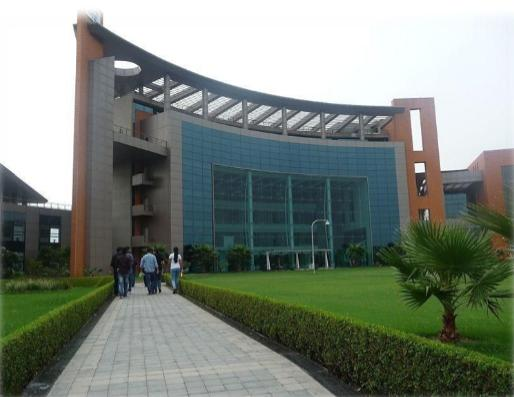
\includegraphics[width=3.5in, height=3in]{images/company.jpg}
	\caption{STMicroelectronics Pvt. Ltd., Greator Noida}
\end{figure}
\noindent STMicroelectronics is a world leader in providing the semiconductor solutions that make a positive contribution to people's lives, today and into the future.\\
\noindent Offering one of the industry's broadest product portfolios, ST serves customers across the spectrum of electronics applications with innovative semiconductor solutions for Smart Driving and the Internet of Things. By getting more from technology to get more from life, ST stands for life.augmented.
\begin{itemize}
	\item Among the world's largest sermicondutor companies.
	\item A leading Integrated Device Manufacturer serving all electronics segments.
	\item A leading technology innovator (approximately 8,300 people working in R\&D, ~15,000 owned patents in ~9,000 patent families and 500 new patent filings).
	\item Delivering solutions that are key to Smart Driving and Internet of Things.
	\item Rich, balanced portfolio (ASICs, Application-Specific Standard Products and Multi-Segment Products).
	\item A pioneer and visionary leader in sustainibility.
	\item Corporate Headquarters: Geneva, Switzerland.
	\item President and CEO: Carlo Bozotti.
	\item 2015 revenue: \$6.90 billion.
	\item Approximately 43,200 employees.
	\item Over 75 sales \& marketing offices in 35 counteries.
	\item 11 main manufacturing sites.
	\item Public ince 1994 - traded on New York Stock Exchange (NYSE: STM), Euronext Paris, and Borsa Italiana.
	\item Created as SGS-THOMPSON Microelectronics in June 1987, from merger of SGS Microelettronica (Italy) and Thomson Semiconducteurs (France).
	\item Renamed STMicroelectronics in May 1998.
\end{itemize}

	\newpage

	\chapter{Introduction to Project}
The SPIRIT is a very low-power RF transceiver, intended for RF wireless applications in the sub-1 GHz band. It is designed to operate both in the license-free ISM and SRD frequency bands at 169, 315, 433, 868, and 915 MHz, but can also be programmed to operate at other additional frequencies in the 300-348 MHz, 387-470 MHz, and 779-956 MHz bands. The air data rate is programmable from 1 to 500 kbps. 
\section{Overview} 
\noindent SPIRIT2 follows the IEEE802.15.4 protocols. IEEE standard 802.15.4 intends to offer the fundamental lower network layers of a type of wireless personal area network (WPAN) which focuses on low-cost, low-speed ubiquitous communication between devices. It can be contrasted with other approaches, such as Wi-fi, which offer more bandwidth and require more power. The emphasis is on very low cost communication of nearby devices with little to no underlying infrastructure, intending to exploit this to lower power consumption even more. The basic framework conceives a 10-meter communications range with a transfer rate of 250 kbit/s. Tradeoffs are possible to favor more radically embedded devices with even lower power requirements, through the definition of not one, but several physical layers. Lower transfer rates of 20 and 40 kbit/s were initially defined, with the 100 kbit/s rate being added in the current revision. IEEE 802.25.4 includes the lower layer i.e; PHY and MAC layer. 6lowPAN sits on the top of the wpan devices and act as the convergence layer to be used by the normal IPv6 kernel stack. 6LowPAN transparently handles the fragmentation and defragmentation between the different maximum transmission units(MTU’s) (127 vs 1280) as well as compressions.\\
\noindent The host system must be able to communicate with SPIRIT in order to set straight the relationships and interaction between various portions of the stack. These communications are of course handled by the Operating System. Furthermore for the OS to communicate with an external peripheral, device drivers are employed. And this is the whole idea of this project: creating a device driver for SPIRIT so that it can be used in conjunction with systems running on Linux based operating systems.\\
\noindent The device driver ensures that the peripheral is able to communicate with the host but the way this communication is to be conducted depends on what physical connection options are offered by the peripheral. In case of the SPIRIT the physical interface is SPI. Once the means of communication are fixed, there comes the question of deciding which part of the protocol is to reside on which side the host or the peripheral. It will be seen in later chapters as to how the whole stack has been fragmented in this project.\\
\noindent Linux is written in C and so are the device drivers for Linux. 
\section{Existing system}
\noindent WPAN has been a prominent technology in networking and has been the backbone of many user applications. As such it only makes sense that an operating system incorporates enough attention to WPAN as a technology. And this is exactly the case with Linux. It was realized early on that WPAN is going to be a major player and hence efforts were made to have it be an integral part of Linux. The software side of WPAN is official WPAN protocol stack for Linux i.e. linux-wpan which will be looked at in later sections of this report. The other major thing that then remains is the hardware: the SPIRIT. Due to increase in number of interconnect devices these days there is a greater need of software infrastructure to support these devices .Since the underlying hardware is a RF Device, and Linux is the Freely available OS with a large base of community support it is dire necessity to develop a Linux RF driver for the ST’s Sub-Ghz hardware – SPIRIT1 and SPIRIT2.\\
\noindent This is of course possible because Linux, the OS has a stack support for SPI, so once a hardware is detected then all that remains is to bridge this stack to the device using some standard protocol. All of this is taken care by the device driver for that particular device. It is simple, in order for a device to be supported, there has to be a device driver for it, and in this section. I describe some of the widely used WPAN devices that are supported by Linux at the time this writing:\\
like Android, Meego ,Moblin ,RT-Linux and to larger base of Interconnect devices running Linux – Like routers, network hubs, IoT devices and wearables. at86rfxxx, mrf24j40, cc2520.
\subsection{ATMEL at86rf230}
The AT86RF230 is a low-power 2.4 GHz radio transceiver which is developed by the ATMEL. Atmel Corporation is an American-based designer and manufacturer of semiconductors, founded in 1984. The company focuses on embedded systems built around microcontrollers. at86rf230 especially designed for ZigBee/IEEE 802.15.4 applications. The AT86RF230 follows the SPI for the communication with the OS. All RF-critical components except the antenna, crystal and de-coupling capacitors are integrated on-chip. This single-chip radio transceiver provides a complete radio transceiver interface between the antenna and the microcontroller. It comprises the analog radio transceiver and the digital demodulation including time and frequency synchronization, and data buffering. In June 2014 they provide the software support for their device in linux. The low power consumption of the device make it highly popular for the linux OS and after that atmel developed many version of this transceiver(under this series at86rfxx).
\begin{figure}[ht]
	\centering
	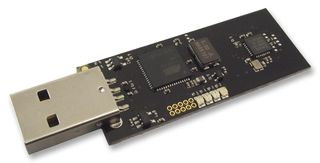
\includegraphics[scale=0.8]{images/atmel.jpg}
	\caption{atmel transceiver}
\end{figure}
\subsection{Microchip mrf24j40}
The MRF24J40 is an IEEE 802.15.4 Standard com­pliant 2.4 GHz RF transceiver. It is the product of Microchip. Microchip Technology is an American manufacturer of microcontroller, memory and analog semiconductors. Its products include microcontrollers (PIC micro, PIC32) Serial EEPROM devices, Serial SRAM devices, radio frequency (RF) devices. It integrates the PHY and MAC functionality in a single chip solution. The MRF24J40 creates a low-cost, low-power, low data rate (250 or 625 kbps) Wireless Personal Area Network (WPAN) device. The MRF24J40 interfaces to many popular Microchip PIC microcontrollers via a 4-wire serial SPI interface, interrupt, wake and Reset pins.\\ 
\noindent The MRF24J40 is compatible with Microchip's ZigBee, MiWi and MiWi P2P software stacks. It works in various mode but the IEEE 802.15.4 feature is supported only in normal mode and each TX FIFO has a specific purpose depending on if the mrf24j40 is configured for beacon and non-beacon-enabled mode. Microchip offers this transceiver in various OS. 
\begin{figure}[ht]
	\centering
	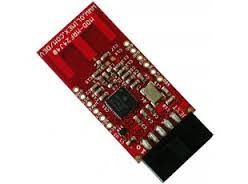
\includegraphics[scale=0.8]{images/microchip.jpg}
	\caption{Microchip transceiver}
\end{figure}
\subsection{Texas CC2520}
The CC2520 is TI's second generation ZigBee IEEE 802.15.4 RF transceiver for the 2.4 GHz unlicensed ISM band. Texas Instruments Inc. (TI) is an American technology company that designs and manufactures semiconductors, which it sells to electronics designers and manufacturers globally headquartered in Dallas, Texas, United States, TI is one of the top ten semiconductor companies worldwide, based on sales volume. This chip enables industrial grade applications by offering state-of-the-art selectivity/co-existence, excellent link budget, operation up to 125°C and low voltage operation. CC2520 has 6 GPIO pins that can be individually configured as inputs, outputs and activate pull-up resistors. There are other solutions by Texas for Wpan as well and they work well with Linux as the driver is there for them.

\begin{figure}[ht]
	\centering
	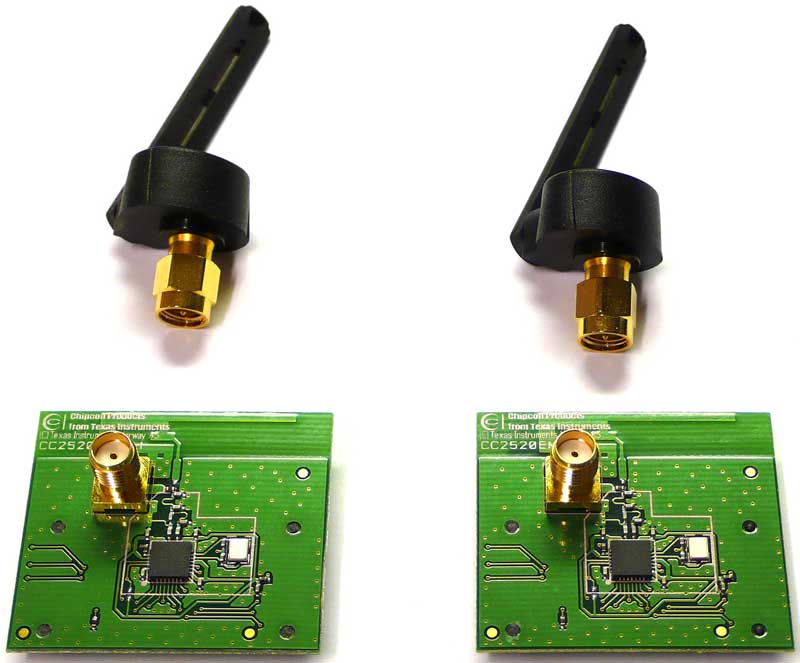
\includegraphics[scale=0.3]{images/texas.jpg}
	\caption{Texas transceiver}
\end{figure}
\section{Requirement Analysis}
There are many wpan adapters out there that have well documented and tested support in Linux based operating systems. Linux being an open source kernel is always inviting people to look into its internal working and stack flow in order to contribute in it.\\
STMicroelectronics excels at grabbing newer opportunities and always be ready with solutions that are on par or even transcends other solutions in the market in a wide range of technologies. The Wpan technology is no different. ST has its fair share of Wpan modules. But thing to be considered here is that even though ST has a wide range of Wpan solutions, none has Linux support.\\ 
So the major requirement of this project was to take a Wpan transceiver by ST and add its support to Linux. And again Linux being open source makes the job much simpler. The module that was considered is the SPIRIT2 transceiver which is SPI based. So the whole requirement of this project can be summed up as adding support (writing a device driver) in Linux (because it is open source and one of the most popular OS kernels in the world) for the Wpan module offered by STMicroelectronic i.e. SPIRIT1 and SPIRIT2.\\
In order to fulfill the above stated requirement it is essential to look into both sides of the coin: Linux driver development and how is the wpan stack being represented there; and then SPIRIT and what portion of the stack is on it and how much of it is needed in order to work with Linux.\\
As SPIRIT2 follows the IEEE 802.1.4 protocols. 802.15.4 covers the lower layer the physical layer and the medium acess control but the good news here is that in linux already there is a support of 802.15.4 so we have to write the driver for our device and then registered that device on the IEEE 802.15.4 platform, for that we have to we have to look into the physical layer i.e. RF layer.\\ 
Another important point to consider is that how the connection is to be made between the Host (running on Linux) and SPIRIT2. SPIRIT2 is based on Serial Peripheral Interface, and in linux already there is the support for Serial peripheral interface so that is exactly what is required to be used for the connections. 
\section{Feasbility Study}
As stated in the requirement analysis section, there are two things that are needed to be considerd here:
\subsection{Does SPIRIT support what wpan offers?}
The answer is yes. Wpan follows the IEEE802.15.4. These are the specification from the IEEE's 802.15 working group, which tackles wireless "personal area" networks, or WPANs. The standard defines a physical-layer and media access control specification, meaning that it covers the frequencies and negotiation options of the connection, but not the protocols that run above it. The communication between between the two spirit is to be held through the 6lowpan these are also the standard developed by the IETF.\\
The 6LoWPAN concept originated from the idea that "the Internet Protocol could and should be applied even to the smallest devices and in linux already there is a support for the 6lowpan because many transceiver from other manufacturer stated early follows the 6lowpan for communications. We will discussed later that how the frame format for transmission of Ipv6 packets as well as well the formation Ipv6 link-local addresses and statelessly auto configured data on the top of IEE802.15.4 networks. Since Ipv6 support of packet size much larger than the largest IEEE802.15.4 frame size, an adaption layer is defined. 
\subsection{Does Linux supports what SPIRIT used to communicate?}
SPIRIT is based on SPI. Any form of communication between the host and SPIRIT is to be had through the Serial Peripheral Interface. There are many SPI based driver in Linux for the wpan.   There are also many network drivers that allow the communication between the host and the controller through SPI. So following the same footsteps it should be possible to send commands from the host to the controller using SPI.\\
Considering the above things, it seems feasible to write a driver for SPIRIT in Linux. The driver shall essentially act as a bridge between SPIRIT protocol stack residing partly in the user space and partly in the kernel space of Linux and SPIRIT.
\section{Objectives of the Project}
\begin{itemize}
	\item To setup a SPIRIT driver interface for SPI.
	\item To make a entry for SPIRIT in sysfs.
	\item To map the IEEE 802.15.4 commands with the SPIRIT2.
	\item To interface the SPI Commands from SPIRIT to host.
\end{itemize}

	\newpage

	\chapter{Product Design}
\section{Wireless Personal Area Network}
WPAN \textbf{(wireless personal area network)} is a personal area network- a network for interconnecting devices centered around an individual person's workspace in which the connections are wireless. Typically, a wireless personal area network uses some technology that permits communication within about 10 meters - in other words, a very short range.\\
Wireless PAN is based on the standard \textbf{IEEE 802.15.4}. A WPAN could serve to interconnect all the ordinary computing and communicating devices that many people have on their desk or carry with them today; or it could serve a more specialized purpose such as allowing the surgeon and other team members to communicate during an operation. There are also many other existing standard such as the IEEE802.11 which is the (wireless local area network) WLAN so why there is a need to developed the new standards so the answer is simple that it requires less power, lesser  bandwidth, has low penetration.
\subsection{Limitations}
WPAN has been designed with some specific fundamentals that happen to serve in a lot of application fields. But this does not means  that it is not apt other kind of applications. Most of its limitations are due to the following two fundamental fact
\begin{enumerate}
	\item The maximum therotical throughput is i\textbf{500Kbps} which is reduces by several factors to only \textbf{5-10KBps} in most cases.
	\item The operating range is generally \textbf{2-5 meters}. This can be extended to \textbf{30 meters} or so but that will of course demand higher strain on the battery life of the devices. This is the defining thing about the BLE technology that the devices are mostly passive in nature and hence it becomes very important for them to have large battery life. In some cases it is seen that the device’s battery can actually outlast other hardware in the device itself.
	\item The loss of the data in WLAN goes upto \textbf{60} which is much higher than that of the WPAN ahich have only \textbf{30} data loss.
	\item Frankly speaking, there is no much benefits of Wireless personal area network over wireless local area network \textbf{WLAN}the WLAN consumes more power because it transmits the data for a longer distance and have the throughput upto 10Mbps. WPAN useful for the short distance communication and low data transmission.
\end{enumerate}
\subsection{WPAN Architecture}
\subsubsection{Application layer}  The upper layer containing most of the application logic, that is used to transfer the data. 6loWPAN is the mostly used upper layer.
\subsubsection{Host} It Contains all the lower layer protocols like PHY and MAC layer in WPAN IEEE802.15.4 acts as the host.
\subsubsection{Controller}  Linux acts as the controller for WPAN.
We will discuseed all these layer one by one so first we start with host because it acts on the ground means it contains the RF layer.
\subsection{IEEE 802.15.4 Network Topologies}
Network topology defines the way in which different devices (under different roles) interact with one another to exchange data through transceiver. These topologies are defined under the specification and are maintained under the IEEE guidelines.\\
Depending on the application requirements, an IEEE 802.15.4 LR-WPAN operates in either of two topologies:
\begin{enumerate}
	\item Star topology.
	\item Peer to Peer topology.
\end{enumerate}
Let's take a look ate each of them individually.
\subsubsection{Star Topology}
In the star topology, the communication is established between devices and a single central controller, called the PAN coordinator. A device typically has some associated application and is either the initiation point or the termination point for network communications. A PAN coordinator can also have a specific application, but it can be used to initiate, terminate, or route communication around the network. The PAN coordinator is the primary controller of the PAN
All devices operating on a network of either topology have unique addresses referred to as extended addresses we will discussed it later that what is extended address. A device will use either the extended address for direct communication within the PAN or the short address that was allocated by the PAN coordinator when the device associated. The PAN coordinator will often be mains powered, while the devices will most likely be battery powered. Applications that benefit from a star topology include home automation, personal computer (PC) peripherals, games, and personal health care.
\begin{figure}[ht]
	\centering
	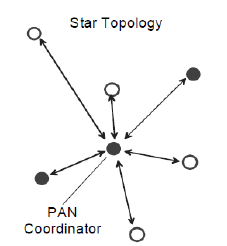
\includegraphics[scale=1.2]{images/star_topology.png}
	\caption{Star topology}
\end{figure}
\subsubsection{Peer to Peer Topology}
The peer-to-peer topology also has a PAN coordinator; however, it differs from the star topology in that any device is able to communicate with any other device as long as they are in range of one another. Peer-to-peer topology allows more complex network formations to be implemented, such as mesh networking topology. Applications such as industrial control and monitoring, wireless sensor networks, asset and inventory tracking, intelligent agriculture, and security would benefit from such a network topology. A peer-to-peer network allows multiple hops to route messages from any device to any other device on the network. Such functions can be added at the higher layer, but they are not part of this standard. Each independent PAN selects a unique identifier. This PAN identifier allows communication between devices within a network using short addresses and enables transmissions between devices across independent networks. The mechanism by which identifiers are chosen is outside the scope of this standard.
\begin{figure}[ht]
	\centering
	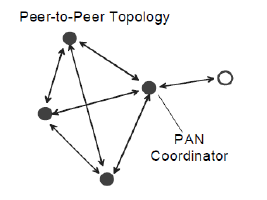
\includegraphics[scale=1]{images/peertopeertopology.png}
	\caption{Peer to Peer topology}
\end{figure}
\subsection{Network formation}
\subsubsection{Star network formation}
After an FFD is activated, it can establish its own network and become the PAN coordinator. All-star networks operate independently from all other star networks currently in operation. This is achieved by choosing a PAN identifier that is not currently used by any other network within the radio communications range. Once the PAN identifier is chosen, the PAN coordinator allows other devices, potentially both FFDs and RFDs, to join its network.
\subsubsection{Peer to Peer network formation}
In a peer-to-peer topology, each device is capable of communicating with any other device within its radio communications range. One device is nominated as the PAN coordinator, for instance, by virtue of being the first device to communicate on the channel. Further network structures are constructed out of the peer-to peer topology, and it is possible to impose topological restrictions on the formation of the network.\\
An example of the use of the peer-to-peer communications topology is the \textbf{cluster tree}. The cluster tree network is a special case of a peer-to-peer network in which most devices are FFDs. An RFD connects to a cluster tree network as a leaf device at the end of a branch because RFDs do not allow other devices to associate. Any FFD is able to act as a coordinator and provide synchronization services to other devices or other coordinators. Only one of these coordinators is the overall PAN coordinator, potentially because it has greater computational resources than any other device in the PAN. The PAN coordinator forms the first cluster by choosing an unused PAN Identifier and broadcasting beacon frames to neighbouring devices.
\begin{figure}[ht]
	\centering
	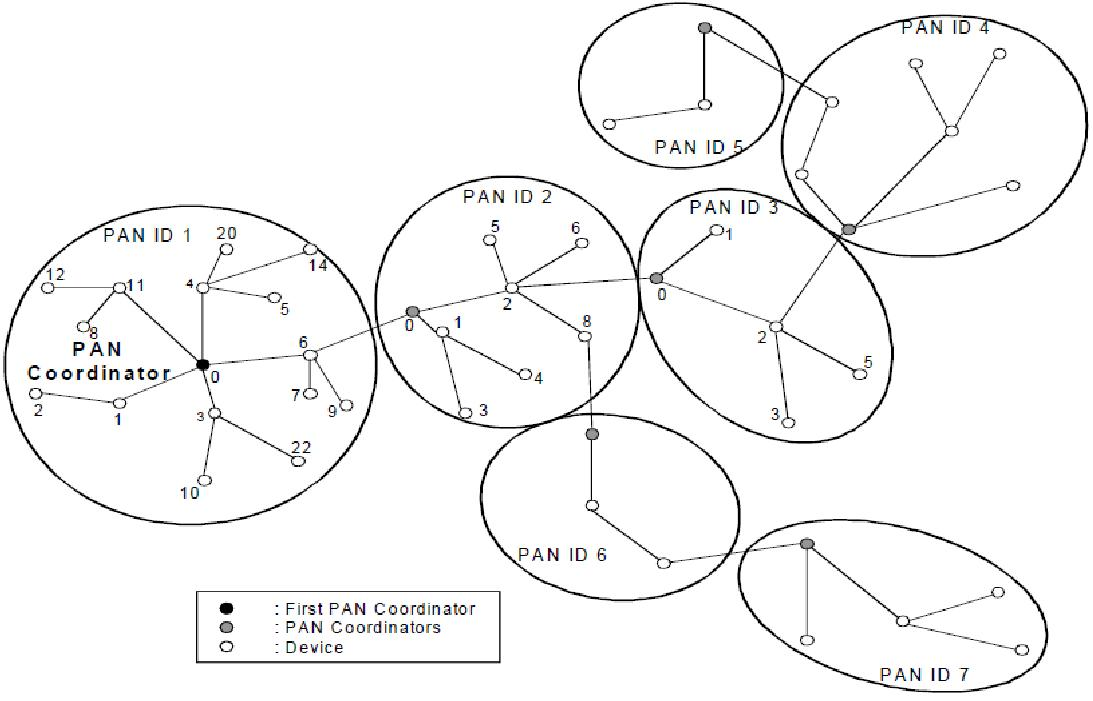
\includegraphics[scale=0.4]{images/cluster_tree.png}
	\caption{Cluster network}
\end{figure}
\section{IEEE 802.15.4 Architecture}
The IEEE 802.15.4 architecture is defined in terms of a number of blocks in order to simplify the standard. These blocks are called layers. Each layer is responsible for one part of the standard and offers services to the higher layers. As OSI have 7 layer but the IEEE 802.1.5.4 constitutes only the lower two layer\\
\begin{enumerate}

	\item{Physical layer(PHY)}
	\item{Medium access control(MAC) layer}
\end{enumerate}
	An LR-WPAN device comprises at least one PHY, which contains the radio frequency (RF) transceiver along with its low-level control mechanism, and a MAC sublayer that provides access to the physical channel for all types of transfer.



\begin{figure}[ht]
	\centering
	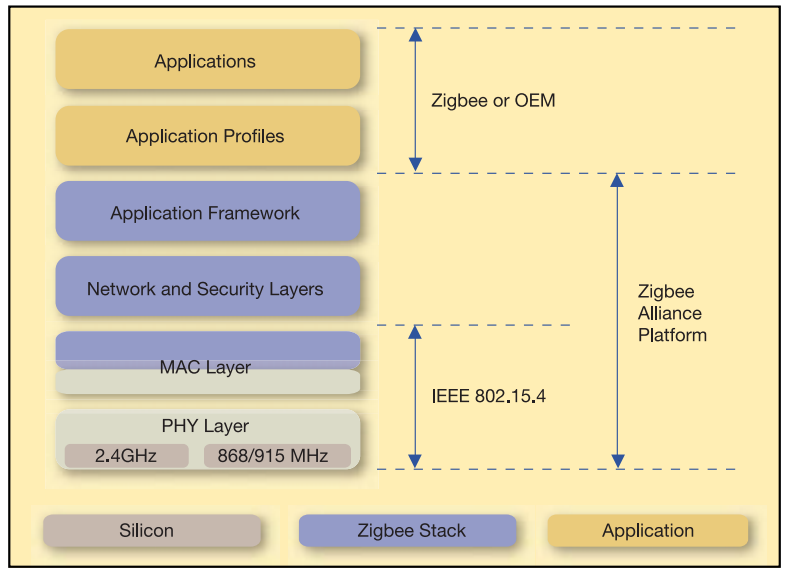
\includegraphics[scale=0.7]{images/ieee.png}
	\caption{IEEE 802.15.4}
\end{figure}
The upper layers, shown in figure, consist of a network layer, which provides network configuration, manipulation, and message routing, and an application layer, which provides the intended function of the device. The upper layer covered by the 6loWPAN. We will discussed the upper layers function in the coming chapter.
\subsection{Physical layer}
The physical layer is the first layer of the Open System Interconnection Model (OSI Model). The physical layer deals with bit-level transmission between different devices and supports electrical or mechanical interfaces connecting to the physical medium for synchronized communication.\\
The PHY is responsible for the following tasks:\\
\begin{enumerate}
	\item{Activation and deactivation of the radio transceiver}
	\item {Energy detection (ED) within the current channel}
	\item {Link quality indicator (LQI) for received packets}
	\item {Clear channel assessment (CCA) for carrier sense multiple access with collision avoidance\textbf{(CSMA/CA)}}
	\item {Channel frequency selection}
	\item{Data transmission and reception}
	\item{Precision ranging for ultra-wide band\textbf{(UWB)}PHY's}
\end{enumerate}
The PHYs defined in this standard are:\\
O-QPSK PHY: \\Direct sequence spread spectrum (DSSS) PHY employing offset quadrature phase shift keying (O-QPSK) modulation, operating in the 780 MHz bands, 868 MHz, 915 MHz, and 2450 MHz.\\
BPSK PHY: \\DSSS PHY employing binary phase-shift keying (BPSK) modulation, operating in the 868 MHz, 915 MHz, and 950 MHz bands.\\
ASK PHY: \\Parallel sequence spread spectrum (PSSS) PHY employing amplitude shift keying.\\
ASK and BPSK modulation, operating in the 868 MHz and 915 MHz bands.\\
CSS PHY: \\Chirp spread spectrum (CSS) employing differential quadrature phase-shift keying.\\
DQPSK:\\  DQPSK modulation, operating in the 2450 MHz band.\\
UWB PHY: \\Combined burst position modulation (BPM) and BPSK modulation, operating in the sub-gigahertz and 3–10 GHz bands.\\
MPSK PHY: \\M-ary phase-shift keying (MPSK) modulation, operating in the 780 MHz.\\
GFSK PHY: \\Gaussian frequency-shift keying (GFSK), operating in the 950 MHz band.\\
\subsection{Operating frequency range}
A compliant device shall operate in one or several frequency bands using the modulation and spreading formats. Devices shall start in the PHY mode in which they are instructed to start. If the device is capable of operating in the 868 MHz or 915 MHz bands using one of the optional PHYs and, it shall be able to switch dynamically between the optional PHY and the mandatory BPSK PHY in that band when instructed to do so. If the 950 MHz band is supported, then at least one of the 950 MHz band PHYs shall be implemented.
\subsection{Medium Acess Control}
The Media Access Control Layer is one of two sublayers that make up the Data Link Layer of the OSI model sublayer handles all access to the physical radio channel and is responsible for the following tasks:
\begin{enumerate}
	\item{Generating network beacons if the device is a coordinator}
	\item{Synchronizing to network beacons}
	\item{Supporting PAN association and disassociation}
	\item{Supporting device security}
	\item{Employing the CSMA-CA mechanism for channel access}
	\item{Handling and maintaining the GTS mechanism}
	\item{Providing a reliable link between two peer MAC entities}
\end{enumerate}
There are two device types:\\ 
Full-function device (FFD)\\ 
Reduced-function device (RFD)\\ 
The FFD may operate in three modes serving as a personal area network (PAN) coordinator, a coordinator, or a device. An RFD shall only operate as a device.
\subsubsection{MAC Services}
The MAC sublayer provides an interface between the next higher layer and the PHY. The MAC sublayer conceptually includes a management entity called the mac layer management activity (MLME). This entity provides the service interfaces through which layer managementons may be invoked. The MLME is also responsible for maintaining a database of managed objects pertaining to the MAC sublayer. This database is referred to as the MAC sublayer PIB.
\begin{figure}[ht]
	\centering
	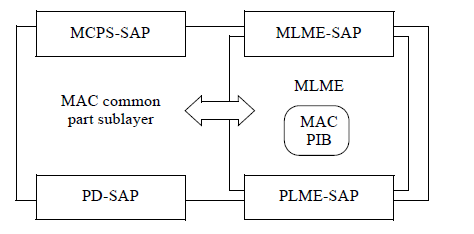
\includegraphics[scale=1]{images/macsublayer.png}
	\caption{MAC Sublayer reference model}
\end{figure}
\subsection{Security}
The MAC sublayer is responsible for providing security services on specified incoming and outgoing frames when requested to do so by the higher layers. The 802.15.4 standard supports the following security services:
\begin{enumerate}
	\item{Data confidentiality}
	\item{Data authenticity}
	\item{Replay protection}
\end{enumerate}
A device may optionally implement security. A device that does not implement security shall not provide a mechanism for the MAC sublayer to perform any cryptographic transformation on incoming and outgoing frames nor require any PIB attributes associated with security. A device that implements security shall provide a mechanism for the MAC sublayer to provide cryptographic transformations on incoming and outgoing frames using information in the PIB attributes associated with security only if the macSecurityEnabled attribute is set to TRUE.\\
\subsection{MAC layer advertising and scanning}
The advertising packets are used to either broadcast data for applications or to discover slaves and to connect to them. The advertising of packets is done aftmake a entry for S2-LP in sysfs.er certain intervals and if during this interval some device is scanning then that device will be able to receive the advertising packet.\\
The advertising packets are used to either broadcast data for applications or to discover slaves and to connect to them. The advertising of packets is done after make a entry for S2-LP in sysfs after certain intervals and if during this interval some device is scanning then that device will be able to receive the advertising packet.\\
The specification defines the two types of scanning\\
\subsubsection{Passive Scanning}
The scanner simply listens for advertising packets, and the advertiser is never aware of the fact that one or more packets were actually received by a scanner.
\subsubsection{Active Scanning}
The scanner issues s Scan Request packet after receiving an advertising packet. The advertiser receives it and responds with a Scan Response packet. This additional packet doubles the effective payload that the advertiser is able to send to the scanner, but it is important to note that this does not provide a means for the scanner to send any user data at all to the advertiser.\\
Before commencing an active or passive scan, the MAC sublayer shall store the value of macPANId and then set it to 0xffff for the duration of the scan this enables the receive filter to accept all beacons. On completion of the scan, the MAC sublayer shall restore the value of macPANId to the value stored before the scan began.
\section{Low Wireless Personal Area Network}
The 6LoWPAN group has defined encapsulation and header compression mechanisms that allow IPv6 packets to be sent and received over IEEE 802.15.4 based networks. IPv4 and IPv6 are the work horses for data delivery for local-area networks, metropolitan area networks, and wide-area networks such as the Internet. Likewise, IEEE 802.15.4 devices provide sensing communication-ability in the wireless domain. The inherent natures of the two networks though, are different.
\subsection{Transmission of IPv6 Packets over IEEE 802.15.4 Networks}
The 6loWPAN sits over the IEEE802.15.4 packets, which acts as the convergence layer for the packet transmission.
\begin{figure}[ht]
	\centering
	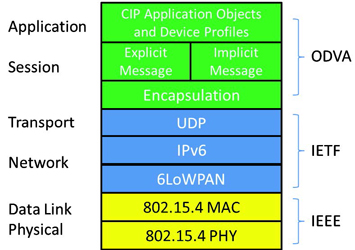
\includegraphics[scale=1]{images/6LoWPAN.png}
	\caption{6 LoWPAN over IEEE}
\end{figure}
\subsection{IEEE 802.15.4 Mode over IPv6} 
IEEE 802.15.4 defines four types of frames\\
\begin{enumerate}
	\item{Beacon frames}
	\item{MAC command frames}
	\item{Acknowledgement frames}
	\item{Data frames}
\end{enumerate}
IPv6 packets MUST be carried on data frames. Data frames may optionally request that they be acknowledged. IEEE 802.15.4 networks can either be nonbeacon-enabled or beacon-enabled.  The latter is an optional mode in which devices are synchronized by a so-called coordinator's beacons.  This allows the use of superframes within which a contention-free Guaranteed Time Service (GTS) is possible. In nonbeacon-enabled networks, data frames (including those carrying IPv6 packets) are sent via the contention-based channel access method of unslotted CSMA/CA. In nonbeacon-enabled networks, beacons are not used for synchronization. However, they are still useful for link-layer device discovery to aid in association and disassociation events.
\subsection{Addressing Modes}
IEEE 802.15.4 defines several addressing modes, it allows the use of either:\\
1. IEEE 64-bit extended addresses or (after an association event)\\
2. 16-bit addresses unique within the PAN.\\
6loWPAN supports both the addresses. Short addresses being transient in nature, a word of caution is in order. Since they are doled out by the PAN coordinator function during an association event, their validity and uniqueness is limited by the lifetime of that association.
\subsection{Maximum transmission Unit}
The MTU size for IPv6 packets over IEEE 802.15.4 is 1280 octets. However, a full IPv6 packet does not fit in an IEEE 802.15.4 frame. 802.15.4 protocol data units have different sizes depending on how much overhead is present.  Starting from a maximum physical layer packet size of 127 octets (aMaxPHYPacketSize) and a maximum frame overhead of 25 (aMaxFrameOverhead), the resultant maximum frame size at the media access control layer is 102 octets. Link-layer security imposes further overhead, which in the maximum case (21 octets of overhead in the AES-CCM-128 case, versus 9 and 13 for AES-CCM-32 and AES-CCM-64, respectively) leaves only 81 octets available.  This is obviously far below the minimum IPv6 packet size of 1280 octets. Furthermore, since the IPv6 header is 40 octets long, this leaves only 41 octets for upper-layer protocols, like UDP.  The latter uses 8 octets in the header which leaves only 33 octets for application data.  Additionally, there is a need for a fragmentation and reassembly layer, which will use even more octets.\\
\begin{enumerate}
	\item{The adaptation layer must be provided to comply with the IPv6 requirements of a minimum MTU.  However, it is expected that}
	\begin{itemize}
		\item Most applications of IEEE 802.15.4 will not use such large packets.
		\item Small application payloads in conjunction with the proper header compression will produce packets that fit within a single IEEE 802.15.4 frame.  The justification for this adaptation layer is not just for IPv6 compliance, as it is quite likely that the packet sizes produced by certain application exchanges (e.g., configuration or provisioning) may require a small number of fragments.
		\end{itemize}
	\item{Even though the above space calculation shows the worst-case scenario, it does point out the fact that header compression is compelling to the point of almost being unavoidable.  Since we expect that most (if not all) applications of IP over IEEE 802.15.4 will make use of header compression.}
\end{enumerate}
\begin{figure}[ht]
	\centering
	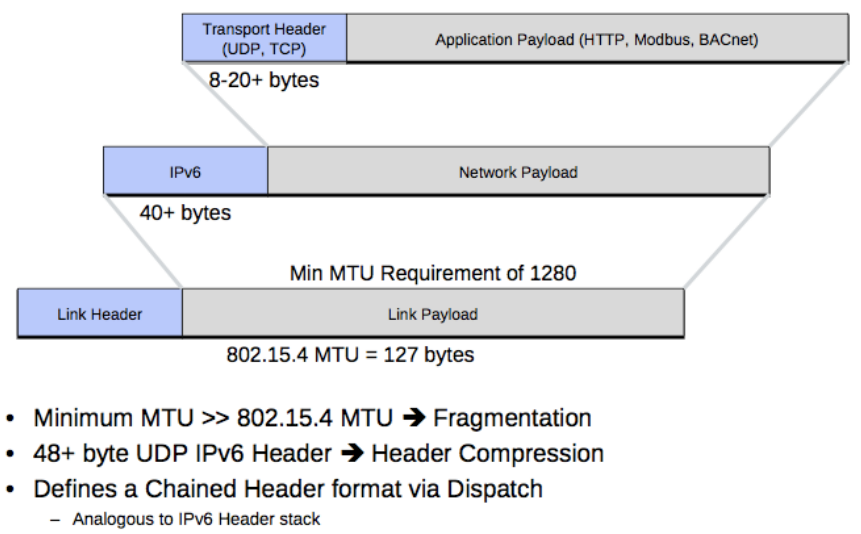
\includegraphics[scale=0.51]{images/headercompression.png}
	\caption{Fragmentation and defragmentation}
\end{figure}
\subsection{Security of IPv6}
The method of derivation of Interface Identifiers from EUI-64 MAC addresses is intended to preserve global uniqueness when possible. However, there is no protection from duplication through accident or forgery. Neighbor Discovery in IEEE 802.15.4 links may be susceptible to threats.  Mesh routing is expected to be common in IEEE 802.15.4 networks. This implies additional threats due to ad hoc routing.  IEEE 802.15.4 provides some capability for link-layer security. Users are urged to make use of such provisions if at all possible and practical.  Doing so will alleviate the threats stated above. \\A sizeable portion of IEEE 802.15.4 devices is expected to always communicate within their PAN (i.e., within their link, in IPv6 terms).  In response to cost and power consumption considerations, and in keeping with the IEEE 802.15.4 model of ``Reduced Function Devices'' (RFDs), these devices will typically implement the minimum set of features necessary.  Accordingly, security for such devices may rely quite strongly on the mechanisms defined at the link layer by IEEE 802.15.4.  The latter, however, only defines the Advanced Encryption Standard (AES) modes for authentication or encryption of IEEE 802.15.4 frames, and does not, in particular, specify key management (presumably group oriented).  Other issues to address in real deployments relate to secure configuration and management. Whereas such a complete picture is out of the scope of this document, it is imperative that IEEE 802.15.4 networks be deployed with such  considerations in mind.  Of course, it is also expected that some IEEE 802.15.4 devices (the so-called ``Full Function Devices'', or ``FFDs'') will implement coordination or integration functions.  These may communicate regularly with off-link IPv6 peers (in addition to the more common on-link exchanges).  Such IPv6 devices are expected to secure their end-to-end communications with the usual mechanisms (e.g., IPsec, TLS, etc).
\section{WPAN The official Linux S2-LP stack}
\textbf{WPAN}is the official Linux personal area protocol stack. It is an Open Source project distributed under the GNU General Public License (GPL).
\begin{figure}[ht]
	\centering
	
\includegraphics[scale=1]{images/linux.png}
	\caption{WPAN the official S2-LP stack of Linux}
\end{figure}
\subsection{History}
The linux-WPAN project was started in 2008. Initially, it was started with the name of linux-zigbee but this name is little confusing because there is no zigbee protocol at all and  Linux is an open source wheras zigbee is managed by zigbee community. The lower layer consist of the PHY and MAC layer as we discussed above and the transport layer consist of the Zigbee protocol.
\begin{figure}[ht]
	\centering
	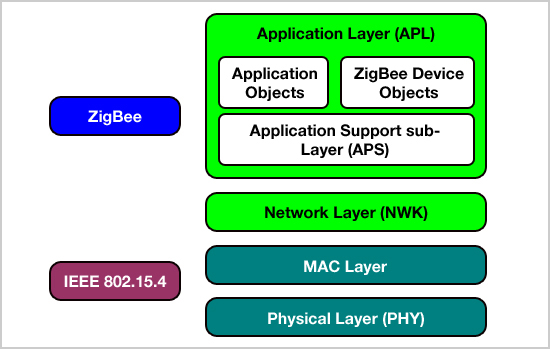
\includegraphics[scale=0.8]{images/WPAN.png}
	\caption{Linux-WPAN}
\end{figure}
Mainly Community slowly took over and the new open standard was formed to avoid confusion with the name linux-WPAN and the new maintainer were Alexander Aring and Pengutronix. Now there are many higher layer protocols which make the use of IEEE 802.15.4 profiles.\\
These are discussed below:\\
\begin{enumerate}
	\item{Zigbee}
	\begin{itemize}
		\item Zigbee Alliance's mesh networking protocol but it’s not available under the GPL licensing as we discussed above.
	\item{MiWi Mesh and MiWi P2P}
		\item Microchip's proprietary mesh and P2P protocols. This protocol is only compatible with the Microchip’s component and they have their own standard.
	\item{6LoWPAN}
		\item IPv6 over 802.15.4.
	\item{WirelessHART}
		\item It’s mainly used for Industrial Automation purpose because it required the more power and data sent by this protocol is of higher bits.
	\end{itemize}
\end{enumerate}
So we have only one option left i.e. IPv6 over 802.15.4.\\
But many of the protocols of the linux-WPAN is taken from the linux-WLAN. If we compare both of the frameworks then.\\ \\
\begin{table}[ht]
	\centering
	\scalebox{1.2}{
	\begin{tabular}{|K{2.2cm} | K{8cm} | K{2.2cm}|}
		\toprule
		\rowcolor{Gray}
		\textbf{WPAN} & \textbf{Description} & \textbf{WLAN} \\
		\hline
		WLAN & Default interfacing naming & WPAN \\
		\hline
		station & Default interfacing type registration & node \\
		\hline
		iw & command framework & iWPAN \\
		\hline
		nl80211 & Netlink kernel framework & nl802154 \\
		\hline
		cfg80211 & Soft and Hard-MAC Interface & cfg802154 \\
		\bottomrule
	\end{tabular}}
	\caption{WLAN and WPAN framework}
\end{table}
\section{S2-LP}
The S2-LP is a narrow band ultra-low power RF transceiver, intended for RF wireless applications in the sub-1 GHz band. It is designed to operate in both the license-free ISM and SRD frequency bands at 433,868 and 920 MHz, but can also be programmed to operate at other additional frequencies in the 430-470 MHz, 860-940 MHz bands. The S2-LP supports different modulation schemes: 2(G)FSK, 4(G)FSK, OOK and ASK. The air data rate is programmable from 0.3 to 500 kbps. The S2-LP can be used in systems with channel spacing of 12.5/25 kHz, complying with the EN 300 220 standard and satisfying the latest FCC narrow banding mandate.
The S2-LP shows a RF link budget higher than 140dB for long communication range and meets the regulatory requirements applicable in territories worldwide, including Europe, Japan, China and USA. The S2-LP integrates a configurable baseband modem with proprietary fully programmable packet format allowing also:
\begin{enumerate}
	\item{IEEE 802.15.4g full hardware packet supporting whitening, CRC, FEC and dual SYNC
	word detection.}
	\item{Wireless M-Bus standard compliance packet format (all performance classes).
	In order to reduce the overall system power consumption and increase the communication reliability, the S2-LP provides an embedded programmable automatic packet acknowledgment, automatic packet retransmission, CSMA/CA engine, low duty cycle protocol, RX sniff mode and timeout protocol. The S2-LP fully supports antenna diversity with an integrated antenna switching control algorithm. Transmitted/received data bytes are buffered in two different 128 bytes FIFOs (TX FIFO and RX FIFO), accessible via SPI interface for host processing. In addition the reduction of external components enables easily and fast integrate the S2-LP on products to enable a short time to market.}
\end{enumerate}
\subsection{Block diagram of S2-LP}
The receiver architecture is low-IF conversion, the received RF signal is amplified by a two-stage lownoise amplifier (LNA) and down-converted in quadrature (I and Q) to the intermediate frequency (IF). LNA and IF amplifiers make up the RX front-end (RXFE) and have programmable gain. The transmitter part of the S2-LP is based on direct synthesis of the RF frequency. The power amplifier (PA) input is the LO generated by the RF synthesizer, while the output level can be configured between -30 dBm and +14 dBm (+16 dBm in boost mode), at pin level with 0.5 dB steps. The data to be transmitted can be provided by an external MCU either through the 128-byte TX FIFO writable via SPI, or directly using a programmable GPIO pin.\\
The S2-LP supports frequency hopping, TX/RX and antenna diversity switch control, extending the link range and improving performance. The S2-LP has a very efficient power management (PM) system. An integrated switched mode power supply (SMPS) regulator allows operation from a battery voltage ranging from +1.8 V to +3.6 V, and with power conversion efficiency of 90percent.
\begin{figure}[ht]
	\centering
	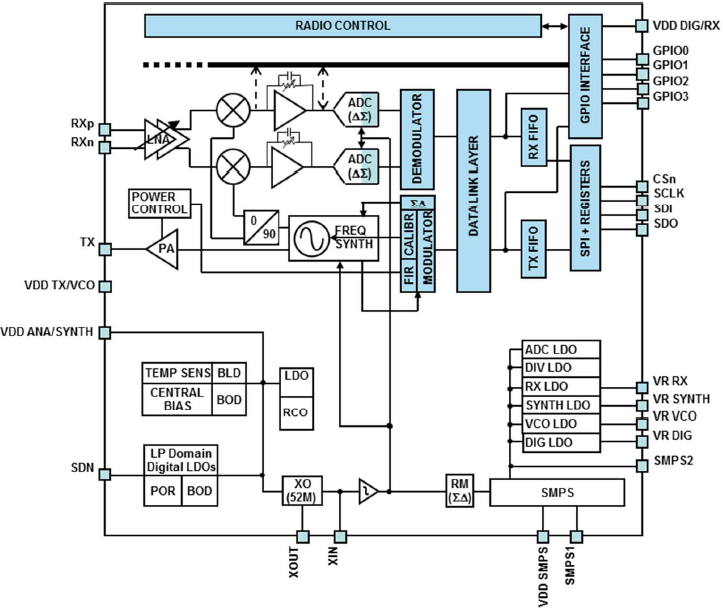
\includegraphics[scale=0.8]{images/spirit.png}
	\caption{Block diagram of S2-LP}
\end{figure}
\subsection{SPIRIT1}
The SPIRIT1 is a very low-power RF transceiver, intended for RF wireless applications in the sub-1 GHz band. It is designed to operate both in the license-free ISM and SRD frequency bands at 169, 315, 433, 868, and 915 MHz, but can also be programmed to operate at other additional frequencies in the 300-348 MHz, 387-470 MHz, and 779-956 MHz bands. The air data rate is programmable from 1 to 500 kbps, and the SPIRIT1 can be used in systems with channel spacing of 12.5/25 kHz, complying with the EN 300 220 standard. It uses a very small number of discrete external components and integrates a configurable baseband modem, which supports data management, modulation, and demodulation.\\
The data management handles the data in the proprietary fully programmable packet format also allows the M-Bus standard compliance format (all performance classes). However, the SPIRIT1 can perform cyclic redundancy checks on the data as well as FEC encoding/decoding on the packets. The SPIRIT1 provides an optional automatic acknowledgement, retransmission, and timeout protocol engine in order to reduce overall system costs by handling all the high-speed link layer operations. Moreover, the SPIRIT1 supports an embedded CSMA/CA engine. An AES 128-bit encryption co-processor is available for secure data transfer. The SPIRIT1 fully supports antenna diversity with an integrated antenna switching control algorithm. The SPIRIT1 supports different modulation schemes: 2-FSK, GFSK, OOK, ASK, and MSK. Transmitted/received data bytes are buffered in two different three-level FIFOs (TX FIFO and RX FIFO), accessible via the SPI interface for host processing.
\subsection{SPIRIT1/S2-LP Protocol Stack}
\begin{figure}[ht]
	\centering
	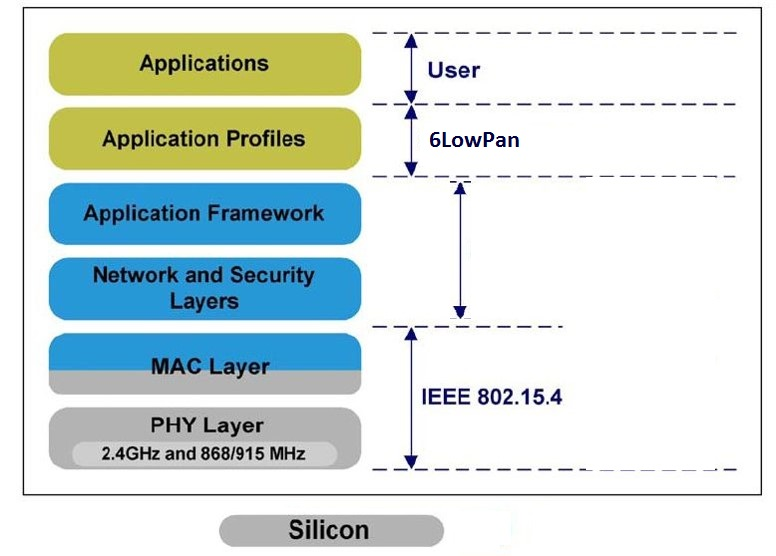
\includegraphics[scale=0.8]{images/protocol.png}
	\caption{SPIRIT1/S2-LP protocol stack}
\end{figure}
Architecture of SPIRIT1 is similar to S2-LP except it does not follows IEEE 802.15.4 stack which is provided by the Linux kernel. If we talk about the protocols and Block Diagram then both are same but the only difference is that S2-LP has 128 bits of FIFO register whereas SPIRIT1 has 96 bits of FIFO register.
\subsection{Pin Diagram of S2-LP}
\begin{figure}[ht]
	\centering
	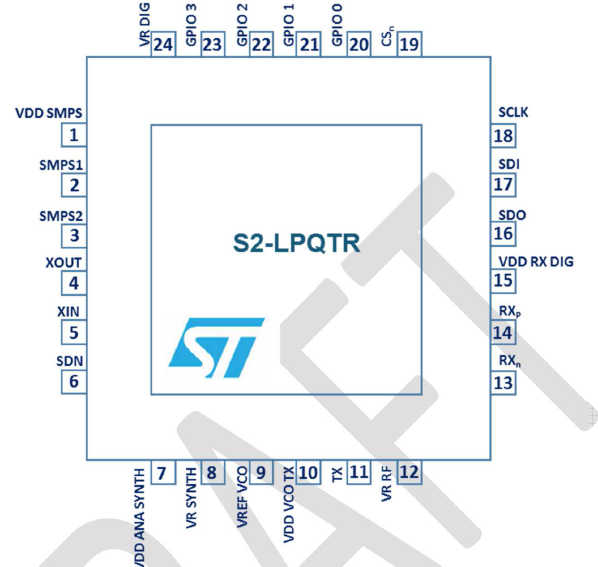
\includegraphics[scale=0.8]{images/pindiagram.png}
	\caption{Pin configuration of S2-LP}
\end{figure}
\subsection{Pin Description}
\begin{table}[ht]
	\centering
	\scalebox{0.8}{
	\begin{tabular}{|K{2cm} | K{4cm} | K{3cm} | K{10cm}|}
		\toprule
		\rowcolor{Gray}
		\textbf{N} & \textbf{Pin Name} & \textbf{Pin type} & \textbf{Description} \\
		\hline
		1 & VDD SMPS & POWER & \\
		\hline
		1 & VDD SMPS & POWER & 1.8 to 3.6 V analog power supply for SMPS only \\
		\hline
		2 & SMPS1 & Analog out & 1.1 to 1.8 V SMPS regulator output to be externally filtered \\
		\hline
		3 & SMPS2 & Analog in & 1.1 to 1.8 SMSP voltage input after LC filtering applied to SMPS1 output \\
		\hline 
		4 & XOUT & Analog out & Crystal oscillator output. connect to an external crystal or leave floating if driving the XIN pin with an external clock \\
		\hline 
		5 & XIN & Analog in & Crystal oscillator input. Connect to an external oscillator or to an external clock source \\
		\hline
		6 & SDN & Digital in & Shutdown input pin. SDN should be =  '0' in all modes but '1' in SHUTDOWN mode \\
		\hline
		7 & VDD ANA/SYNTH & Power & 1.8 to 3.6 V \\
		\hline 
		8 & VR SYNTH & Analog in/out & 1.2 V SYNTH-LDO output for decoupling \\
		\hline
		9 & VREF VCO & Analog out & 1.2 V VCO-LDO for decoupling \\
		\hline
		10 & VDD VCO/TX & Power & 1.8 V to 3.6 V power supply \\
		\hline
		11 & TX & RF output & RF output signal \\
		\hline
		12 & VR RF & Analog in/out & 1.2 V RX-LDO for decoupling \\
		\hline
		13 & RXn & RF in & Differential RF input signals for the LNA \\
		\hline
		14 & RXp & RF in & Differential RF input signals for the LNA \\
		\hline
		15 & VDD RX/DIG & Power & 1.8 to 3.6 V power supply \\
		\hline
		16 & SDO & Digital out & SPI slave data output \\
		\hline
		17 & SDI & Digital In & SPI slave data input \\
		\hline 
		18 & SCLK & Digital in & SPI slave clock input \\
		\hline 
		19 & CSn & Digital in & SPI chip select \\
		\hline
		20 & GPIO0 & Digital I/O & General purpose I/O \\
		\hline 
		21 & GPIO1 & Digital I/O & General purpose I/O \\
		\hline
		22 & GPIO2 & Digital I/O & General purpose I/O \\
		\hline
		23 & GPIO3 & Digital I/O & General purpose I/O \\
		\hline
		24 & VR DIG & Analog in/out & 1.2 V supply for decoupling\\
	\bottomrule
	\end{tabular}}
	\caption{SPIRIT1 pin description}
\end{table}
In this Report we mainly focused for the SPIRIT1 driver writing because I wrote the Driver for SPIRIT1, as we discussed in the previous section that the SPIRIT1 and S2-LP architecture are same except the IEEE protocols.
\subsection{Operating Modes}
Several operating modes are defined for the SPIRIT1:
\begin{itemize}
	\item Reset Mode
	\item Sleep Mode
	\item Standby Mode
	\item Ready Mode
	\item Lock Mode
	\item Shutdown Mode
\end{itemize}
The SPIRIT1 is provided with a built-in main controller which controls the switching between the two main operating modes: transmit (TX) and receive (RX). In shutdown condition (the SPIRIT1 can be switched on/off with the external pin SDN, all other functions/registers are available through the SPI interface and GPIOs), no internal supply is generated (in order to have minimum battery leakage), and hence, all stored data and configurations are lost. The GPIO and SPI ports during SHUTDOWN are in HiZ. From shutdown, the SPIRIT1 can be switched on from the SDN pin and goes into READY state, which is the default, where the reference signal from XO is available. From READY state, the SPIRIT1 can be moved to LOCK state to generate the high precision LO signal and/or TX or RX modes. Switching from RX to TX and vice versa can happen only by passing through the LOCK state. This operation is normally managed by radio control with a single user command (TX or RX). At the end of the operations above, the SPIRIT1 can return to its default state (READY) and can then be put into a sleeping condition (SLEEP state), having very low power consumption. If no timeout is required, the SPIRIT1 can be moved from READY to STANDBY state, which has the lowest possible current consumption while retaining FIFO, status and configuration registers. To manage the transitions towards and between these operating modes, the controller works as a state machine, whose state switching is driven by SPI commands. \\
\begin{figure}[ht]
	\centering
	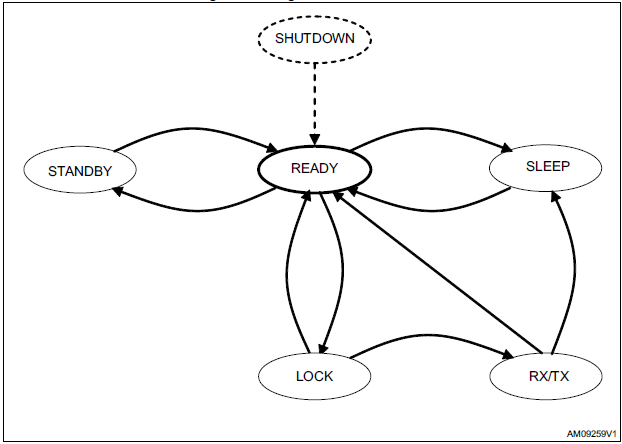
\includegraphics[scale=0.8]{images/modes.png}
	\caption{Operating modes of SPIRIT1}
\end{figure}
The SPIRIT1 radio control has three stable states (READY, STANDBY, LOCK) which may be defined stable, and they are accessed by the specific commands (respectively READY, STANDBY, and LOCKRX/LOCKTX), which can be left only if any other command is used. All other states are transient, which means that, in a typical configuration, the controller remains in those states, at most for any timeout timer duration. Also the READY and LOCK states behave as transients when they are not directly accessed with the specific commands (for example, when LOCK is temporarily used before reaching the TX or RX states).
\begin{figure}[ht]
	\centering
	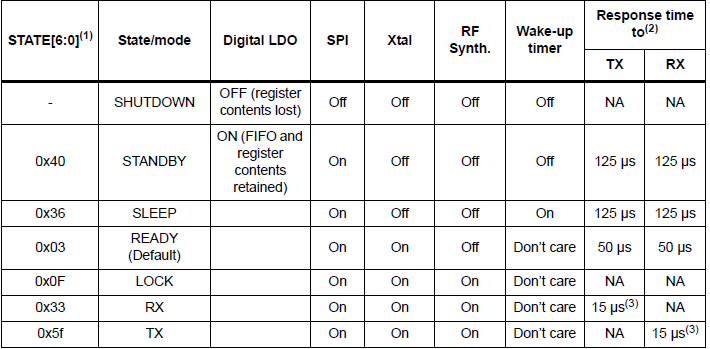
\includegraphics[scale=0.8]{images/table.png}
	\caption{Spirit opearting modes summary}
\end{figure}



	\newpage

	\chapter{Development and Implementation}
\section{The Linux Kernel}
The Linux kernel is a monolithic Unix-like computer operating system kernel. The Linux operating system is based on it and deployed on both traditional computer systems such as personal computers, servers and small system on chip computers; usually in the form of Linux distributions, and on various embedded devices such as routers, wireless access points, PBXes, set-top boxes, FTA receivers, smart TVs, PVRs and NAS appliances. The Android operating system for tablet computers, smartphones and smart-watches is also based atop the Linux kernel.\\
The Linux kernel was conceived and created in 1991 by Linux Torvalds for his personal computer and with no cross-platform intentions, but has since expanded to support to huge array of computer architecture, many more than other operating systems or kernels. Linux rapidly attracted developers and users who adopted it as the kernel for other free software projects, notably the GNU Operating System. The Linux kernel has received contributions from nearly 12,000 programmers from more than 1,200 companies, including some of the largest software and hardware vendors.
\subsection{The Linux Device Driver Model}
Linux today supports more hardware devices than any other operating system in the history of the world. It does this using a development model significantly different from the familiar Windows device driver model. The Linux development process continues to evolve to better support the needs of Independent Hardware Vendors (IHVs), distributions, and other members of the community, and the advantages of the Linux model are increasing with time. While Linux will not provide a stable source or binary interface for driver developers, IHVs should familiarize themselves with a number of useful projects, many sponsored by the Linux Foundation, that ease driver development, including the Hardware NDA program, the Linux Drivers Project, and the Driver Backport Workgroup. When IHVs engage with the Linux community, they almost invariably find that the Linux driver model provides significant benefits that lower their costs while producing better drivers.
\subsubsection{Overview}
A fundamental purpose for operating systems (OSes) is to serve as an abstraction layer between applications and hardware to enable interoperability. An IHV wants their hardware to be able to make use of all the relevant features of an OS, and an OS wants to take full advantage of the hardware it's running on. Since both the OS and the hardware tend to add and to rearrange features over time, it is a dynamic interaction. What everybody wants is for the hardware to “Just Work” without hassles or support calls.\\
Today, Linux works with more devices than any other OS in the history of the world.
\subsubsection{Driver Model}
The Linux driver model is different. For users, the goal is to provide the “Just Works” experience. The Linux model is that IHVs get the source code for their driver accepted into the mainline kernel. This entails a public peer review process to ensure that the driver code is of sufficient quality and does not have obvious bugs or security risks. Linux has neither a stable binary driver ABI nor a stable source-code driver Application Programming Interface (API). That is, there is no guarantee that an interface provided in one version of the kernel will be available in the next version, and portions of the ABI and API change in every kernel release.\\
By contrast, the Linux kernel does provide a stable user-space interface for Linux applications. These applications essentially have a contract with the Linux kernel that the user-space binary interfaces they rely on will continue to work consistently over time. That's why a pre-compiled Linux application can run correctly on multiple distributions and multiple versions. The underlying implementation of the user-space binary interfaces can and does change, but even an application compiled for pre-1.0 Linux will run correctly on the latest kernel. This is the opposite of device drivers, which have no guarantee whatsoever that any interface they rely on, whether binary or source, will remain consistent between versions of the kernel.\\
Counterintuitive though it might be from a proprietary viewpoint, this lack of internal kernel interface stability is preferable because both the kernel code and all of the drivers relying on it are open source. In fact, driver code is an integral part of the Linux operating system, not a second-class add-on. Once a driver is accepted into the mainline kernel, it will be maintained over time as internal kernel interfaces change. That is, when a subsystem maintainer accepts a patch to make an incompatible change to a kernel interface, that patch will simultaneously upgrade every driver that relies on the interface. And, new drivers and any upgrades to them automatically flow downstream from the mainline kernel to all Linux distributions.\\
The key strength of this approach from the user's viewpoint is that, in happy contrast with proprietary operating systems like Windows Vista, once a device is working on a given version of Linux, that support continues through all future versions. (Devices are generally only removed when they have become so rare that no users can be found.) In Linux, hardware support only gets better; it never gets worse.\\
From the IHV's point of view, the big benefit is that an IHV's driver is maintained over time by the community, meaning that other people fix, tune, and add features to the driver. When internal kernel interfaces change in each new OS release, IHVs don't need to write and release a new driver; their driver is upgraded automatically. Obsolete interfaces can be deprecated and removed rather than being maintained indefinitely. Common subsystems can be factored out of drivers, enabling leaner, less buggy device drivers while adding more functionality for all hardware. This improves the stability, security, and maturity of both the OS and the driver.\\
In addition, the Linux model enables cross-architecture driver support nearly for free. Even when an IHV only tests their driver on one chip architecture, interested developers ensure that the driver works with every architecture that Linux supports, which is more than any other OS in history. The strength of this approach has been especially apparent over the last decade as many chip architectures have moved from the 32 to 64 bits. Nearly all Linux drivers were quickly updated to support these newer architectures, while driver support for 64-bit Windows Vista even on the highest volume x86 architecture remains extremely poor today.\\
The biggest hurdle of the Linux driver model for some IHVs is the need to open source their driver code, which a small (but thankfully dwindling) number have been reluctant to do. Also, once a driver is accepted into the mainline, it can take up to 18 months to be deployed into an enterprise distro. It has not until now been convenient to backport the driver to existing distros, but that is improving with the Driver Backport Workgroup.\\
Having hardware reliably supported by Linux means getting the driver accepted into the mainline kernel. Supporting an out-of-mainline open source driver creates significant, never-ending support costs for the IHV, as new versions constantly need to be released as the kernel API changes. Supporting an out-of-mainline binary driver means even bigger, never-ending support costs for the IHV, and directly contradicts the recent statement by a large number of kernel developers that binary drivers are “undesirable”.\\
The Linux driver model is different from the Windows model many IHVs are used to. But it is a consistent and compelling approach, and has been successful at supporting nearly the entire universe of computer hardware. Moreover, the vast majority of all IHVs have adapted to Linux and have thriving businesses that work with the Linux driver development model.
\subsection{Overview of SPI support in Linux}
\subsubsection{What is SPI?}
The "Serial Peripheral Interface" (SPI) is a synchronous four wire serial link used to connect microcontrollers to sensors, memory, and peripherals. It's a simple "de facto" standard, not complicated enough to acquire a standardization body.  SPI uses a master/slave configuration.\\
The three signal wires hold a clock (SCK, often on the order of 10 MHz), and parallel data lines with "Master Out, Slave In" (MOSI) or "Master In, Slave Out" (MISO) signals.  (Other names are also used.)  There are four clocking modes through which data is exchanged; mode-0 and mode-3 are most commonly used.  Each clock cycle shifts data out and data in; the clock doesn't cycle except when there is a data bit to shift.  Not all data bits are used though; not every protocol uses those full duplex capabilities.\\
SPI masters use a fourth "chip select" line to activate a given SPI slave device, so those three signal wires may be connected to several chips in parallel.  All SPI slaves support chipselects; they are usually active low signals, labeled nCSx for slave 'x' (e.g. nCS0).  Some devices have other signals, often including an interrupt to the master. \\
Unlike serial busses like USB or SMBus, even low level protocols for SPI slave functions are usually not interoperable between vendors (except for commodities like SPI memory chips).
\begin{itemize}
	\item SPI may be used for request/response style device protocols, as with touchscreen sensors and memory chips.
	\item It may also be used to stream data in either direction (half duplex), or both of them at the same time (full duplex).
	\item Some devices may use eight bit words.  Others may use different word     lengths, such as streams of 12-bit or 20-bit digital samples.
	\item Words are usually sent with their most significant bit (MSB) first, but sometimes the least significant bit (LSB) goes first instead.
	\item Sometimes SPI is used to daisy-chain devices, like shift registers.
\end{itemize}
In the same way, SPI slaves will only rarely support any kind of automatic discovery/enumeration protocol.  The tree of slave devices accessible from a given SPI master will normally be set up manually, with configuration tables.\\
SPI is only one of the names used by such four-wire protocols, and most controllers have no problem handling "MicroWire" (think of it as half-duplex SPI, for request/response protocols), SSP ("Synchronous Serial Protocol"), PSP ("Programmable Serial Protocol"), and other related protocols.\\
Some chips eliminate a signal line by combining MOSI and MISO, and limiting themselves to half-duplex at the hardware level. In fact some SPI chips have this signal mode as a strapping option.  These can be accessed using the same programming interface as SPI, but of course they won't handle full duplex transfers.  You may find such chips described as using "three wire" signaling: SCK, data, nCSx. (That data line is sometimes called MOMI or SISO.) \\
Microcontrollers often support both master and slave sides of the SPI protocol.  This document (and Linux) currently only supports the master side of SPI interactions.
\subsubsection{Who uses SPI?}
Linux developers using SPI are probably writing device drivers for embedded systems boards.  SPI is used to control external chips, and it is also a protocol supported by every MMC or SD memory card.  (The older "DataFlash" cards, predating MMC cards but using the same connectors and card shape, support only SPI.)  Some PC hardware uses SPI flash for BIOS code. \\
SPI slave chips range from digital/analog converters used for analog sensors and codecs, to memory, to peripherals like USB controllers or Ethernet adapters; and more. \\
Most systems using SPI will integrate a few devices on a mainboard. Some provide SPI links on expansion connectors; in cases where no dedicated SPI controller exists, GPIO pins can be used to create a low speed "bitbanging" adapter.  Very few systems will "hotplug" an SPI controller; the reasons to use SPI focus on low cost and simple operation, and if dynamic reconfiguration is important, USB will often be a more appropriate low-pincount peripheral bus. \\
Many microcontrollers that can run Linux integrate one or more I/O interfaces with SPI modes. Given SPI support, they could use MMC or SD cards without needing a special purpose MMC, SD or SDIO controller.
\subsubsection{The SPI programming interface}
The linux/spi/spi.h header file includes kerneldoc, as does the main source code, and you should certainly read that chapter of the kernel API document.  This is just an overview, so you get the big picture before those details. \\
SPI requests always go into I/O queues.  Requests for a given SPI device are always executed in FIFO order, and complete asynchronously through completion callbacks.  There are also some simple synchronous wrappers for those calls, including ones for common transaction types like writing a command and then reading its response. \\
There are two types of SPI driver, here called: \\
Controller drivers ... controllers may be built into System-On-Chip 	processors, and often support both Master and Slave roles. 	These drivers touch hardware registers and may use DMA. 	Or they can be PIO bitbangers, needing just GPIO pins.\\ 
Protocol drivers ... these pass messages through the controller 	driver to communicate with a Slave or Master device on the 	other side of an SPI link. \\
So for example one protocol driver might talk to the MTD layer to export data to filesystems stored on SPI flash like DataFlash; and others might control audio interfaces, present touchscreen sensors as input interfaces, or monitor temperature and voltage levels during industrial processing. And those might all be sharing the same controller driver.\\
A "struct spi\_device" encapsulates the master-side interface between those two types of driver.  At this writing, Linux has no slave side programming interface. \\
There is a minimal core of SPI programming interfaces, focussing on using the driver model to connect controller and protocol drivers using device tables provided by board specific initialization code.  SPI shows up in sysfs in several locations: 
\begin{itemize}
	\item /sys/devices/.../CTLR ... physical node for a given SPI controller 
	\item /sys/devices/.../CTLR/spiB.C... spi\_device on bus "B", chipselect C, accessed through CTLR. 
	\item /sys/bus/spi/devices/spiB.C ... symlink to that physical .../CTLR/spiB.C device 
	\item /sys/devices/.../CTLR/spiB.C/modalias ... identifies the driver that should be used with this device (for hotplug/coldplug) 
	\item /sys/bus/spi/drivers/D ... driver for one or more spi*.* devices 
	\item /sys/class/spi\_master/spiB ... symlink (or actual device node) to a logical node which could hold class related state for the controller managing bus "B". All spiB.* devices share one physical SPI bus segment, with SCLK, MOSI, and MISO. 
\end{itemize}
Note that the actual location of the controller's class state depends on whether you enabled CONFIG\_SYSFS\_DEPRECATED or not.  At this time, the only class-specific state is the bus number ("B" in "spiB"), so those /sys/class entries are only useful to quickly identify busses.
\section{The C Programming Language}
C is the language of the Linux kernel. Almost all of the kernel and related applications are written in C. C is of course the language of development in this project.\\
C is a general-purpose programming language with features economy of expression, modern flow control and data structures, and a rich set of operators. C is not a ``very high level'' language, nor a ``big''one, and is not specialized to any particular area of application. But its absence of restrictions and its generality make it more convenient and effective for many tasks than supposedly more powerful languages. C was originally designed for and implemented on the UNIX operating system on the DEC PDP-11, by Dennis Ritchie. The operating system, the C compiler, and essentially all UNIX applications programs (including all of the software used to prepare this book) are written in C. Production compilers also exist for several other machines, including the IBM System/370, the Honeywell 6000, and the Interdata 8/32. C is not tied to any particular hardware or system, however, and it is easy to write programs that will run without change on any machine that supports C.\\
The C language has a very simple structure and hence is much easily converted into machine code without any overhead that may be faced when using other languages. That is why almost all of the kernel development and device drivers are done in C language only even after the introduction of so many other versatile languages like C++.
\section{Development Boards}
In order to develop and test the driver code as well as to interface the BlueNRG chip to the host via SPI, there was need for a system-on-board computer. The host of course needed to run on a Linux kernel, so the following two were the obvious choices
\subsection{Raspberry Pi 2}
Several generations of Raspberry Pis have been released. The first generation (Raspberry Pi 1 Model B) was released in February 2012. It was followed by a simpler and inexpensive model Model A. In 2014 the foundation released a board with an improved design in Raspberry Pi 1 Model B+. The model laid the current "mainline" form-factor. Improved A+ and B+ models were released a year later. A cut down "compute" model was released in April 2014, and a Raspberry Pi Zero with smaller size and limited input/output (I/O) and general-purpose input/output (GPIO) abilities was released in November 2015 for US\$5. The Raspberry Pi 2 which added more RAM was released in February 2015. Raspberry Pi 3 Model B released in February 2016 is bundled with on-board WiFi and Bluetooth. As of 2016, Raspberry Pi 3 Model B is the newest mainline Raspberry Pi. These boards are priced between US \$20–35.\\
All models feature a Broadcom system on a chip (SoC), which includes an ARM compatible central processing unit (CPU) and an on chip graphics processing unit (GPU, a VideoCore IV). CPU speed ranges from 700 MHz to 1.2 GHz for the Pi 3 and on board memory range from 256 MB to 1 GB RAM. Secure Digital (SD) cards are used to store the operating system and program memory in either the SDHC or MicroSDHC sizes. Most boards have between one and four USB slots, HDMI and composite video output, and a 3.5 mm phone jack for audio. Lower level output is provided by a number of GPIO pins which support common protocols like I²C. The B-models have an 8P8C Ethernet port and the Pi 3 has on board Wi-Fi 802.11n and Bluetooth.\\
The Foundation provides Raspbian, a Debian-based Linux distribution for download, as well as third party Ubuntu, Windows 10 IOT Core, RISC OS, and specialised media center distributions. It promotes Python and Scratch as the main programming language, with support for many other languages. The default firmware is closed source, while an unofficial open source is available.
The Raspberry Pi 3 model was used for preliminary development of this driver.
\begin{figure}[H]
	\centering
	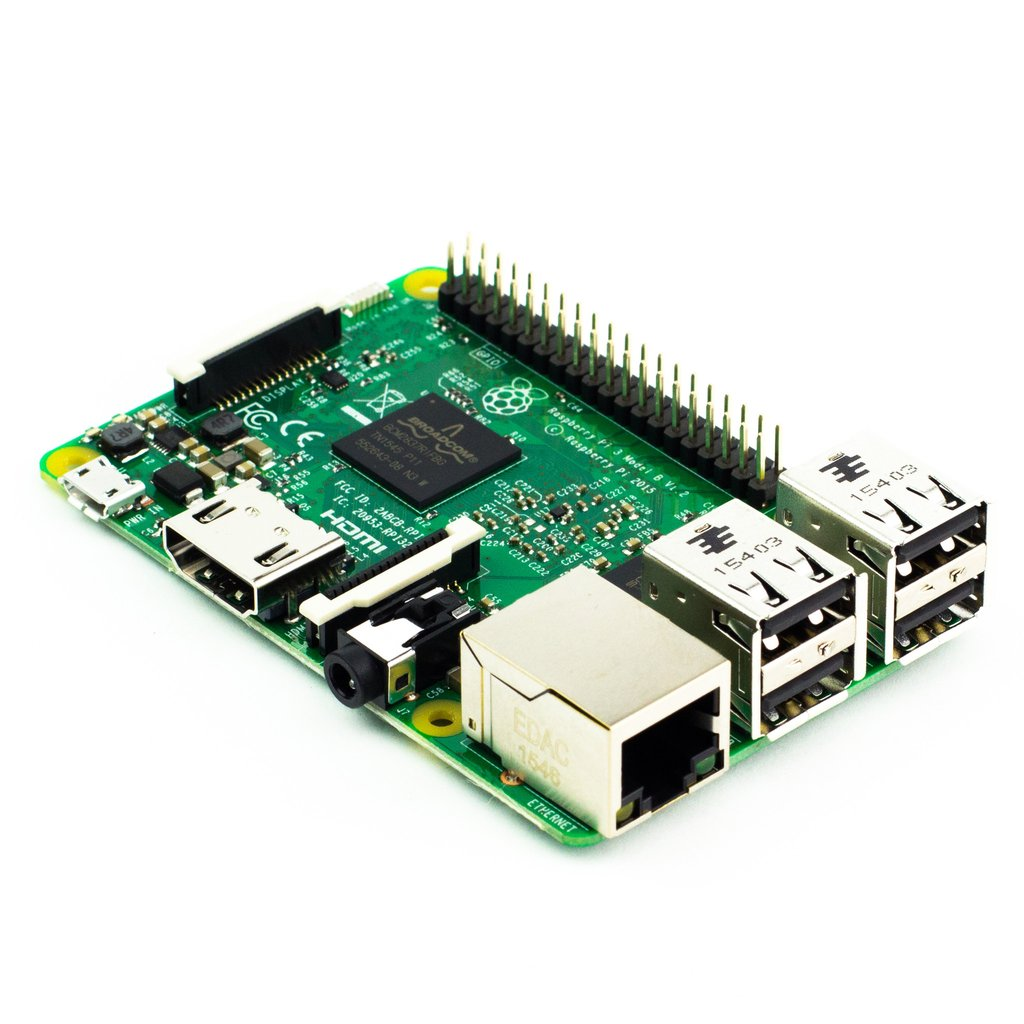
\includegraphics[width=3.5in, height=3in]{images/raspberry_pi.png}
	\caption{Raspberry Pi 2}
\end{figure}
\subsection{BeagleBone Black}
The BeagleBoard is a low-power open-source hardware single-board computer produced by Texas Instruments in association with Digi-Key and Newark element14. The BeagleBoard was also designed with open source software development in mind, and as a way of demonstrating the Texas Instrument's OMAP3530 system-on-a-chip. The board was developed by a small team of engineers as an educational board that could be used in colleges around the world to teach open source hardware and software capabilities. It is also sold to the public under the Creative Commons share-alike license. The board was designed using Cadence OrCAD for schematics and Cadence Allegro for PCB manufacturing; no simulation software was used.\\
The BeagleBone Black is the newest member of the BeagleBoard family. It is a lower-cost, high-expansion focused BeagleBoard using a low cost Sitara XAM3359AZCZ100 Cortex A8 ARM processor from Texas Instruments. It is similar to the Beaglebone,but with some features removed and some features added. The table below gives the high points on the differences between the BeagleBone and BeagleBone Black.
\begin{figure}[ht]
	\centering
	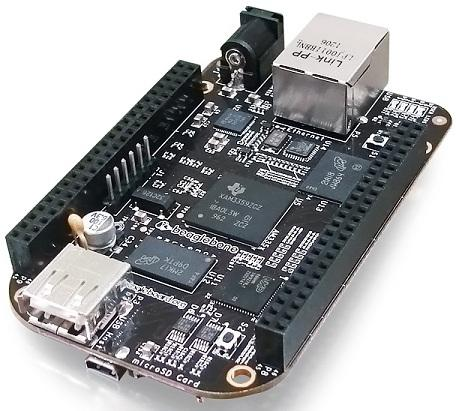
\includegraphics[width=3.5in, height=3in]{images/beaglebone_black.png}
	\caption{BeagleBone Black}
\end{figure}
\section{Tools used}
\subsection{Buildroot}
Buildroot is a set of Makefiles and patches that simplifies and automates the process of building a complete and bootable Linux environment for an embedded system, while using cross-compilation to allow building for multiple target platforms on a single Linux-based development system. Buildroot can automatically build the required cross-compilation toolchain, create a root file system, compile a Linux kernel image, and generate a boot loader for the targeted embedded system, or it can perform any independent combination of these steps. For example, an already installed cross-compilation toolchain can be used independently, while Buildroot only creates the root file system. \\
Buildroot is primarily intended to be used with small or embedded systems based on various computer architectures and instruction set architectures (ISAs), including x86, ARM, MIPS and PowerPC. Numerous architectures and their variants are supported; Buildroot also comes with default configurations for several off-the-shelf available embedded boards, such as Cubieboard, Raspberry Pi and SheevaPlug. Several third-party projects and products use Buildroot as the basis for their build systems, including the OpenWrt project that creates an embedded operating system, and firmware for the customer-premises equipment (CPE) used by the Google Fiber broadband service.\\
Multiple C standard libraries are supported as part of the toolchain, including the GNU C Library, uClibc and musl, as well as the C standard libraries that belong to various preconfigured development environments, such as those provided by Linaro. Buildroot's build configuration system internally uses Kconfig, which provides features such as a menu-driven interface, handling of dependencies, and contextual help; Kconfig is also used by the Linux kernel for its source-level configuration. Buildroot is organized around numerous automatically downloaded packages, which contain the source code of various userspace applications, system utilities, and libraries. Root file system images, which are the final results, may be built using various file systems, including cramfs, JFFS2, romfs, SquashFS and UBIFS.\\
Buildroot is free and open-source software, maintained by Peter Korsgaard and licensed under version 2 or later of the GNU General Public License (GPL). The project started in 2001, with initial intentions to serve as a testbed for uClibc. New releases are made available every three months.
\begin{figure}[ht]
	\centering
	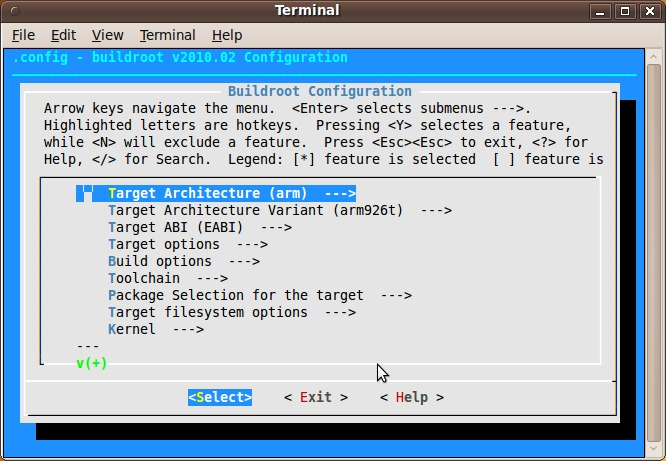
\includegraphics[width=3.5in, height=3in]{images/buildroot.png}
	\caption{Buildroot}
\end{figure}
\subsection{Cscope}
While hacking around the Linux source code it becomes very difficult to keep track of the program flow or the variable structures in your head. There isn’t any IDE to help out in source code browsing either. In such situation a tool is necessary that browses source code and is based on the terminal. This is where cscope comes into picture.\\
cscope is a programming tool which works in console mode, text-based interface, that allows computer programmers or software developers to search source code of the programming language C, with some support for C++ and Java. It is often used on very large projects to find source code, functions, declarations, definitions and regular expressions given a text string. cscope is free and released under a BSD license. The original developer of cscope is \textbf{Joe Steffen}.\\
The history of the tool goes back to the days of the PDP-11, but it is still used by developers who are accustomed to using the vi or Vim editor or other text-based editors, instead of editors based on graphical user interfaces (GUI)s. The functions in cscope are available to varying degrees in modern graphical source editors.
cscope is used in two phases. First a developer builds the cscope database. The developer can often use find or other Unix tools to get the list of filenames needed to index into a file called cscope.files. The developer then builds a database using the command cscope -b -q -k. The k flag is intended to build a database for an operating system or C library source code. It will not look in /usr/include. Second, the developer can now search those files using the command cscope -d. Often an index must be rebuilt whenever changes are made to files.\\
In software development it is often very useful to be able to find the callers of a function because this is the way to understand how code works and what other parts of the program expect from a function. cscope can find the callers and callees of functions, but it is not a compiler and it does that by searching the text for keywords. This has the disadvantages that macros and duplicate symbol names can generate an unclear graph. There are other programs that can extract this information by parsing the source code or looking at the generated object files.
cscope was created to search content within C files, but it can also be used (with some limits) for C++ and Java files.
\begin{figure}[ht]
	\centering
	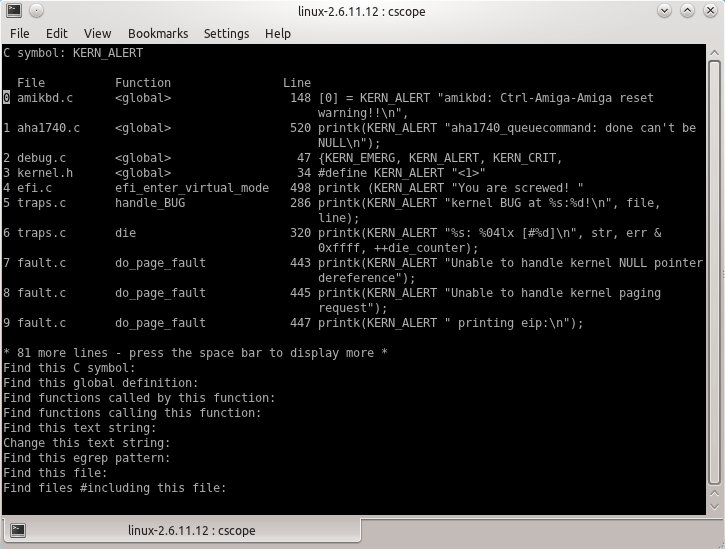
\includegraphics[scale=0.5]{images/cscope.png}
	\caption{Source Browsing through Cscope}
\end{figure}
\subsection{VIM}
Vim (a contraction of Vi IMproved) is a clone of Bill Joy's vi text editor program for Unix. It was written by Bram Moolenaar based on source for a port of the Stevie editor to the Amiga and first released publicly in 1991. Vim is designed for use both from a command-line interface and as a standalone application in a graphical user interface. Vim is free and open source software and is released under a license that includes some charityware clauses, encouraging users who enjoy the software to consider donating to children in Uganda. The license is compatible with the GNU General Public License. Although Vim was originally released for the Amiga, Vim has since been developed to be cross-platform, supporting many other platforms. In 2006, it was voted the most popular editor amongst Linux Journal readers; in 2015 the Stack Overflow developer survey found it to be the third most popular text editor; and in 2016 the Stack Overflow developer survey found it to be the fourth most popular development environment. Although there are many editor available such as Nano. In Vim we have two modes Insert mode and command mode. Insert mode is started by pressing the I and then we insert the words whereas command mode is start by pressing the Esc key.\\
Some basic commands are :
\begin{itemize}
	\item Moving through the text is usually possible with the arrow keys, but in the command mode try:
	\item h to move the cursor to the left
	\item l to move it to the right
	\item k to move up
	\item j to move down
	\item SHIFT-G will put the prompt at the end of the document.
\end{itemize}
\subsection{Logic Analyzer}
A logic analyzer is an electronic instrument that captures and displays multiple signals from a digital system or digital circuit. A logic analyzer may convert the captured data into timing diagrams, protocol decodes, state machine traces, assembly language, or may correlate assembly with source-level software. Logic Analyzers have advanced triggering capabilities, and are useful when a user needs to see the timing relationships between many signals in a digital system.\\
\begin{figure}[ht]
	\centering
	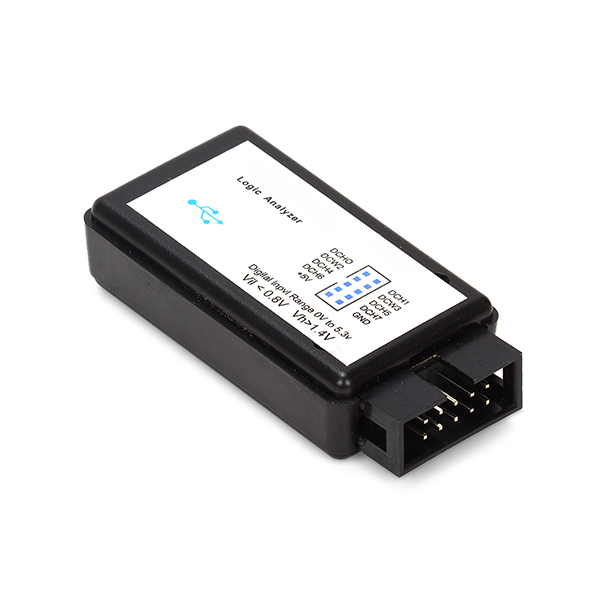
\includegraphics[scale=0.5]{images/logic_analyzer.png}
	\caption{Logic Analyzer}
\end{figure}
\subsection{Programming interface}
\subsubsection{SYSFS programming Interface}
sysfs is a pseudo file system provided by the Linux kernel that exports information about various kernel subsystems, hardware devices, and associated device drivers from the kernel's device model to user space through virtual files. In addition to providing information about various devices and kernel subsystems, exported virtual files are also used for their configuring. sysfs provides functionality similar to the sysctl mechanism found in BSD operating systems, with the difference that sysfs is implemented as a virtual file system instead of being a purpose-built kernel mechanism. Sysfs is used by several utilities to access information about hardware and its driver (kernel modules) such as udev or HAL. Scripts have been written to access information previously obta For every kobject that is registered with the system, a directory is created for it in sysfs. That directory is created as a subdirectory of the kobject's parent, expressing internal object hierarchies to userspace. %Top-level directories in sysfs represent the common ancestors of object hierarchies; i.e. the subsystems the objects belong to. Sysfs internally stores a pointer to the kobject that implements a directory in the kernfs_node object associated with the directory. In the past this kobject pointer has been used by sysfs to do reference counting directly on the kobject whenever the file is opened or closed. With the current sysfs implementation the kobject reference count is only modified directly by the function sysfs_schedule_callback().%
\section{Testing}
The driver job is to send the commands from the one SPIRIT to another one and getting back its response. if all this happen sucessfully then that should means that the SPIRIT is able to communicate with another SPIRIT.\\
For testing the SPIRIT we have to do the following SPIRIT:
\subsection{Enable the SPI in RPI2 board}
	\begin{enumerate}
		\item To enable the SPI in raspberry PI board. Run the following command.
			\textbf{sudo raspi-config}
			\begin{figure}[ht]
				\centering
				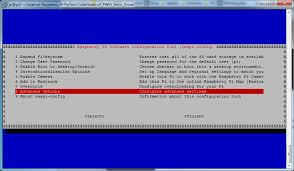
\includegraphics[scale=1.2]{images/spi.png}
				\caption{enable the SPI in RPI2 board}
			\end{figure}
		\item Select the Advanced boot option
		\item Select Enable the SPI and then select on save and exit
	\end{enumerate}
\subsubsection{Make the entry in dts}
Make the entry in dts for the SPIRIT1 under the SPI cateogary.
\subsection{Interfacing between RPI2 and SPSGRF(SPIRIT1)}
The SPSGRF-868 and SPSGRF-915 are easy-to-use, low power sub-GHz modules based on the SPIRIT1 RF transceiver, operating respectively in the 868 MHz SRD and 915 MHz ISM bands.\\
The SPSGRF series enables wireless connectivity in electronic devices, requiring no RF experience or expertise for integration into the final product. As an FCC, IC, and CE certified solution, the SPSGRF series optimizes the time-to-market of end applications. The SPSGRF-915 is an FCC certified module (FCC ID: S9NSPSGRF) and IC certified (IC 8976C-SPSGRF), while the SPSGRF-868 is certified CE0051.
\begin{table}[ht]
	\centering
	\scalebox{1}
	{
		\begin{tabular}{|K{3cm} | K{2cm} | K{5cm}|}
		\toprule
		\rowcolor{Gray}
		\textbf{Pin name} & \textbf{RPI2 pin no.} & \textbf{SPSGRF pin no.} \\
		\hline
		MISO & 19 & 12 \\
		\hline
		MOSI & 21 & 12 \\
		\hline
		SCLK & 23 & 12 \\
		\hline
		CSn & 24 & 12 \\
		\hline
		VSS & 1 & 12 \\
		\hline
		GND & 6 & 12 \\
		\bottomrule
		\end{tabular}
	}
	\caption{RPI2 and SPIRIT Interfacing}
\end{table}
\subsection{Test using logic Analyzer}
We discussed in the previous section about the logic analyzer and how it works. Now we test the SPI of SPIRIT using logic analyzer. It gives us an idea that the data through the SPI is going correctly or not. For that we have to connect the logic Analyzer with the SPIRIT board and send the data over sysfs file using command:\\
\textbf{echo 1 > filename}
Run the above command and notice the data over logic analyzer. It gives:
After the data through the SPI is flowing correctly. Now we have to send the commands for the SPIRIT to become ready. For that we send the command 0x03 over SPI after that SPIRIT become ready to accept the data. 
\subsection{Test the hardware}
When the SPIRIT become ready to accept the data. Now for the hardware verification we have to read the version info and version number of the SPIRIT to verify that whether our hardware is recognised by the Linux or not.
\begin{table}[ht]
	\centering
	\scalebox{0.85}
	{
	\begin{tabular}{|K{5cm} | K{2cm} | K{5cm} | K{2cm} | K{5cm}|}
	\toprule
	\rowcolor{Gray}
	\textbf{Regsiter} & \textbf{Address} & \textbf{Field name} & \textbf{Reset} & \textbf{Description} \\
	\hline
	DEVICEINFO & 0xF0 & PARTNUM & 0x01 & Device part number \\
	\hline
	DEVICEINFO & 0xF1 & VERSION & 0x30 & Device version number \\
	\bottomrule
	\end{tabular}
	}
	\caption{Hardware Register}
\end{table}
Hardware verification means it should give the value 1 of part number and 48 of the version number. When we get this value it means our hardware is recognised by the Linux.






	\newpage

	\chapter{Testing of the driver of LED7708}
\section{LED7708 Introduction}
The LED7708 has been specifically designed to supply several LEDs from a single low-voltage rail in
order to address TV and monitor backlights, medium- and large-size LCD panel backlights and
RGB/RGGB backlight applications. It has sixteen current generators rated at 40 V and a 4-wire serial
interface to control LED brightness. These channels can be put in parallel for higher output currents. A
selectable 12-bit or 16-bit gray-scale brightness control allows independent PWM on each channel. A
programmable on-chip dimming oscillator is provided to simplify external circuitry. The device has
dedicated pins to lock synchronize with other devices (master or slave) for noise reduction in multi-
device applications.\\
The LED7708 implements basic protection (OVP, OCP and thermal shutdown), as well as LED-array
protection. It can detect and manage open-LED and shorted-LED faults, and different fault
management options are available in order to cover most application needs. The board has been
designed as a demonstration of a solution for medium/large LCD panel backlight drivers, but is
suitable for any application involving several LEDs assembled in strings (e.g. advertisement panels,
signs, gaming, etc.).
\subsection{LED7708 read/write protocols}
Protocols for read and write LED7708 registers.
\subsubsection{Serial interface internal registers}
The internal registers are organized in control registers and brightness registers. Access to the desired
register is performed by encoding the destination address via a serial key on the bus (a serial key
consists of a certain number of clock pulses during the high-state of the LE signal). All the internal
registers are 16 bits wide. \\
\begin{table}[ht]
	\centering
	\scalebox{1}
	{
		\begin{tabular}{|K{5cm} | K{5cm}|}
			\toprule
			\rowcolor{Gray}
			\textbf{DCLK rsing edge with LE=1} & \textbf{operation} \\
			\hline
			1 & Data latch \\
			\hline
			2-3 & Global latch \\
			\hline 
			4-5 & Write CHSEL \\
			\hline
			6-7 & Read CHSTA \\
			\hline 
			8-9 & Write DEVCFG \\
			\hline
			10-11 & Read DEVCFG \\
			\hline
			11-12 & Write GSLAT \\
			\bottomrule
		\end{tabular}
	}
		\caption{Internal register operation encoding}
\end{table}
\subsection{LED7708 Linux device driver}
Below is the Linux kernel Architecture showing where all the basic components and their
functionality lies and showing where the LED7708 LDD fits in.
\begin{figure}[ht]
         \centering
         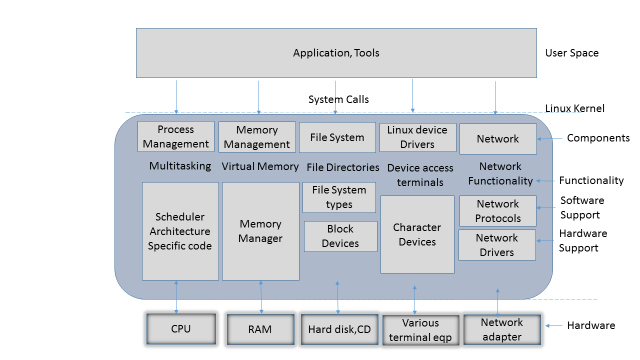
\includegraphics[scale=0.7]{images/kernel.png}
         \caption{Linux kernel architecture}
\end{figure}
\section{Interfacing of the LED7708 with RPI2 board}
\subsection{Hardware setup}
You will need the following items while working with LED7708 with Raspberry Pi 2\\
\begin{enumerate}
	\item \textbf{LED7708} Evaluation Board.
	\item A Connector or Jumper wires to connect LED7708 with the Rpi2 according to the connection
diagram shown in figure below.
	\item Standard HDMI cable for display along with a HDMI Monitor or also can alternatively work
	remotely on PC (Windows or Linux) using any remote terminal Application like Putty.
	\item RS232 FTDI hardware cable for taking serial Logs (Only for taking boot time debugging logs).
	\item Wireless/Wired Keyboard for running the test scripts if working directly (Not remotely) on the
	RPI2 board.
\end{enumerate}
\subsubsection{Hardware connection between LED7708 and RPI2 board}
\begin{figure}[ht]
         \centering
         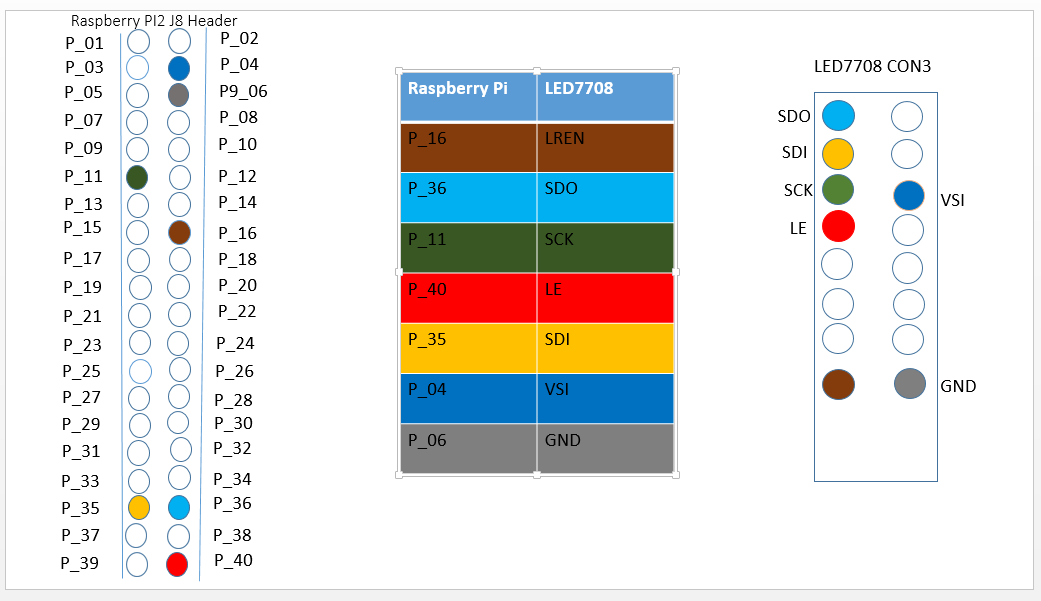
\includegraphics[scale=0.44]{images/raspberryled.png}
         \caption{Interfacing between LED board and RPI2}
\end{figure}
\subsubsection{Hardware Setup between RPI2 and LED7708 Eval board}
\begin{figure}[ht]
         \centering
         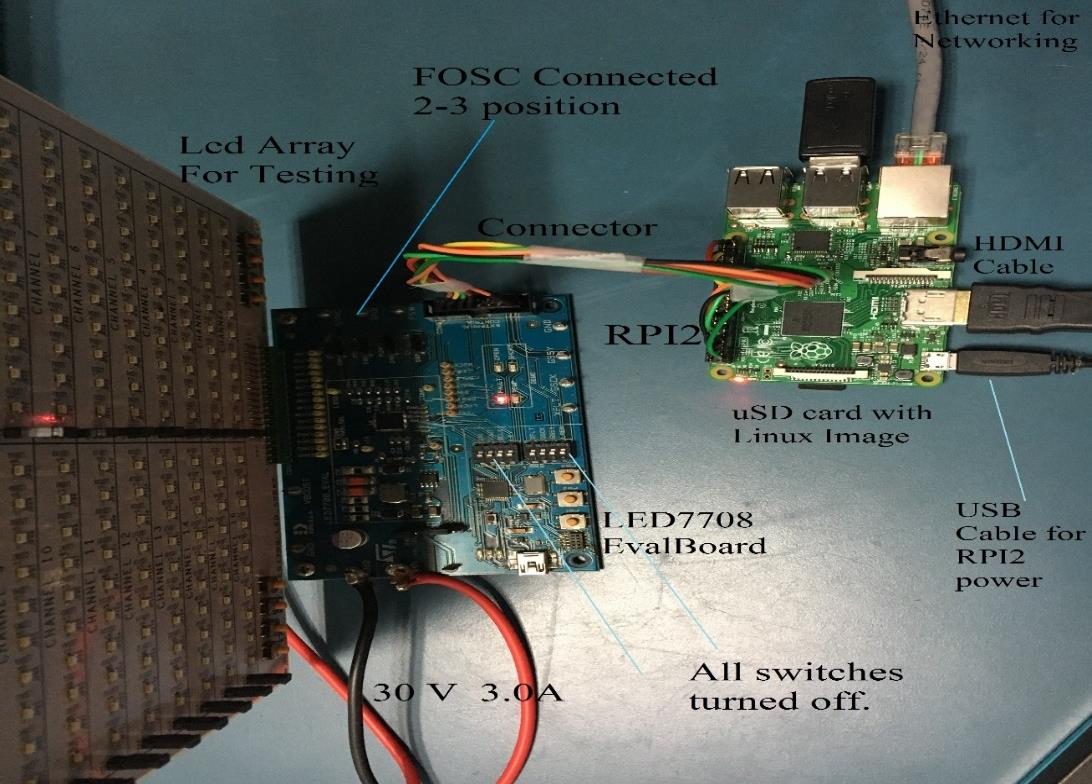
\includegraphics[scale=0.4]{images/raspberryledsetup.png}
         \caption{Hardware setup between LED7708 and RPI2 board}
\end{figure}
\subsection{Software setup}
For integrating the kernel driver with the Raspberry pi we have to bring up the RPI2 with the
appropriate Linux kernel. Please follow the below steps to prepare the RPI2 with Kernel 4.4.23
version.
\begin{enumerate}
	\item Download the kernel source
	Create a directory to store the Raspberry related files (e.g. /home/$<$my pc$>$/rpi2) and run the following
	command in that directory.\\
	git clone https://github.com/raspberrypi/linux.git \\
	if you want to branch to any other kernel run the below command .e.g below command will clone
	4.8.y branch. To see the available branches you can do git branch -a \\
	git checkout -b rpi-4.8.y --track origin/rpi-4.8.y
	\item Download the tool chain
	Tool chain will be required to build/compile the boot loader and the kernel sources.
	Download Raspberry PI cross-compilers by running the following command on your build
	machine.\\
	git clone https://github.com/raspberrypi/tools\\
	\item Configuring the kernel \\
	cd linux\\
	KERNEL=kernel7\\
	make ARCH=arm CROSS\_COMPILE=arm-linux-gnueabihf- bcm2709$_$defconfig
	\item Building the kernel
	Now it's time to build the kernel (image) and modules and .dtbs. Run this command in your terminal
	to build the kernel.\\
	make ARCH=arm CROSS\_COMPILE=arm-linux-gnueabihf- zImage modules dtbs
	\item Flashing the kernel on a new SD card
	Before that if you are using the new SD card you have to flash the NOOB or Raspbian image on it first
	and then follow the below steps.
	\begin{itemize}
		\item Download Raspbian image directly.
		using a computer with an SD card reader, visit the official Raspberry Pi Downloads page.
		\item Click on the Rasbian.
		\item Click on the Download ZIP button under ‘Raspbian Jessie (full desktop image)’, and select a folder
		to save it to.
		\item Extract the files from the zip.
		\item Visit \textbf{etcher.io} and download and install the Etcher SD card image utility.
		\item Run Etcher and select the Raspbian image you unzipped on your computer or laptop.
		\item Select the SD card drive. Note that the software may have already selected the right drive.
		\item Finally, click Burn to transfer Raspbian to the SD card. You'll see a progress bar that tells you how
		much is left to do. Once complete, the utility will automatically eject/unmount the SD card so it's safe
		to remove it from the computer.
	\end{itemize}
\end{enumerate}
\section{Adding Linux Device driver support in the Linux kernel}
Adding a LDD support in the Linux kernel means adding its source code in the Linux kernel. This
can be done either dynamically (building the driver as a module – out of the tree kernel
building) or by compiling the driver along with the kernel sources (in built driver). Also before
that Hardware (LED7708) specific parameters (like interface signals with the Raspberry PI)
needs to be defined to the kernel in the device tree of the platform in which LED7708 needs to
be interfaced.
\subsection{Adding Device tree bindings for LED7708 device driver}
Adding Device tree bindings for the Led7708 Linux driver.\\
In $<$path\_to\_kernel$>$/arch/arm/boot/dts/\\
nano bcm2709-rpi-2-b.dts\\
In this file make the entry for the led7708 board in the led class.\\
\subsection{Adding Linux driver in the kernel - Out of the tree}
Use the below Makefile to build the module.\\
\#MODULES := leds-st.o\\
ARCH := arm\\
CROSS\_COMPILE := arm-linux-gnueabihf-\\
obj-m := \$(MODULES)\\
OUTDIR := /$<$path to built kernel$>$/linux/\\
MAKEARCH := \$(MAKE) ARCH=\$(ARCH) CROSS\_COMPILE=\$(CROSS\_COMPILE)\\
all: modules\\
modules:\\
\$(MAKEARCH) -C \$(OUTDIR) M=\${shell pwd} modules\\
clean:\\
\$(MAKEARCH) -C \$(OUTDIR) M=\${shell pwd} clean\\
\section{Insert the modules}
Modules can be inserted using the commands \\
insmod leds-st.ko\\
Once the module is inserted successfully you can see the sysfs being created in the led directory and there is the sixteen channels for the leds class which you can access
directly and build your application by accessing them.\\
Example wave forms for the below sequence of commads:\\
\begin{itemize}
	\item W(08,04,2130)
	\item W(08,04,8440)
	\item W(04,04,FFFF)
	\item W(08,04,2131)
	\item W(02,04,FFFF)
\end{itemize}
Running the following scripts give the below waveform.
\begin{figure}[ht]
         \centering
         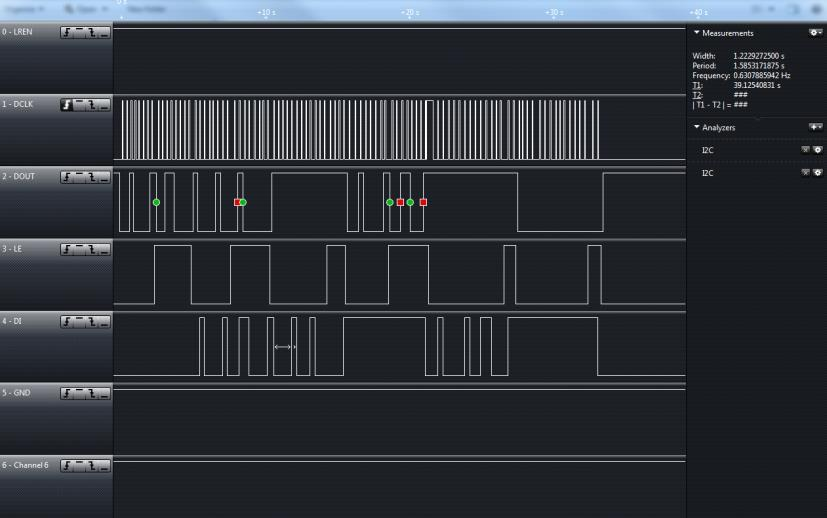
\includegraphics[scale=0.5]{images/waveform.png}
         \caption{Wave form for the example script}
\end{figure}









	\newpage

	\chapter{Conclusion and Future Scope}
\section{Conclusion}
I have learnt a great deal working on this project. The learning was not limited to project only but the whole experience of working as an intern in a multinational company like STMicroelectronics was immensely educational. Being an intern, one is always challenged by the fundamental difference between classroom coaching and real industrial experience. But such a challenge is exactly the purpose of six months training.\\
The whole experience of working on this project and contributing in a few others has been very rewarding as it has given great opportunities to learn new things and get a firmer grasp on already known technologies. Here is a reiteration of some of the technologies I have encountered, browsed and learnt:
\begin{itemize}
	\item Operating System: \textbf{Linux}
	\item Language: \textbf{C}
	\item Development Host: \textbf{Raspberry Pi}, \textbf{BeagleBone Black}
	\item Integrated Build Environment: \textbf{Buildroot}
\end{itemize}
So during this project I learnt all the above things. Above all I got to know how software is developed and how much work and attention to details is required in building even the most basic of components of any project. Planning, designing, developing code, working in a team, testing, etc. these are all very precious lessons in themselves. 
\section{Future Scope}
SPIRIT1 is a relatively new technology. This implies that there is a long road ahead of more features, more research and more hardware for this technology. As such there is always room for inclusion in the Linux kernel for all of this. If the completely new hardware is introduced then it becomes very important to have its driver included in Linux. This is not just have the support for the device in Linux but it also acts like an endorsement for the device that its driver has been registered with the coveted Linux kernel.\\
Talking specifically about some of the other solutions by ST, following two come to immediate consideration that can also be driven by a Linux host by means of device driver written in a manner much similar to SPIRIT:
\begin{enumerate}
	\item \textbf{SPIRIT 1}
	\item \textbf{S2-LP}
\end{enumerate}
The continuous need for more software related to SPIRIT1 in Linux is not just restricted to device driver development. WPAN is the official stack for Linux but even it does not implement everything in the WPAN we have to include the features of the IEEE 802.15.4. Some features are missing and are intended for the future. Also since with new specification releases, more and more features get introduced into the technology. So the stack will also have to sustain with the specification. Some of the things that are not yet implemented in WPAN but are part of the IEEE 802.15.4:
\begin{itemize}
	\item New netlink framework nl802154 
	\item Privacy
	\item IEEE802154 cryptography layer on top of nl802154
	\item Improvements in frame parsing and creation
	\item Better connection management between linux and other OS such as Contiki
\end{itemize}

	\newpage


	\begin{thebibliography}{9}
	\bibitem{IEEE 802.15.4}\textbf{IEEE802.15.4 specification}\\\textit{http://standards.ieee.org/getieee802/download/802.15.4-2006.pdf}\\
	\bibitem{Driver Book}\textbf{Linux Device Drivers}, 4th edition\\
		a book by \textit{Jonathan Corbet, Alessandro Rubini}, and \textit{Greg Kroah-Hartman}.
	\bibitem{Linux kernel Documentation}\textbf{Linux Kernel Documentation for device drivers}.
	\bibitem{Data sheet}\textbf{SPIRIT1 datasheet}\\
		\textit{http://www.st.com/content/ccc/resource/technical/document/datasheet/68/6c/7b/ec/b2/6b/49/16/DM00047607.pdf/files/DM00047607.pdf/jcr:content/translations/en.DM00047607.pdf}
	\bibitem{Build the kernel}\textbf{Build the kernel for BBB}\\\textit{https://eewiki.net/display/linuxonarm/BeagleBone+Black}\\
\end{thebibliography}

\end{document}
